% \documentclass tells LaTeX what type of document you are creating.
% report is suitable for theses, dissertations, and project reports because it supports chapters.
% 12pt sets the default font size to 12 points.
% a4paper sets the paper size to A4 (210 × 297 mm).
\documentclass[12pt,a4paper]{report}
% -------------------------------
% PACKAGES
% -------------------------------
% Enable UTF-8 character encoding
\usepackage[utf8]{inputenc}
% Use Times font
\usepackage{times}
% Control line spacing
\usepackage{setspace}
% Insert and manage images
\usepackage{graphicx}
% Default folder for image files
\graphicspath{{figures/}}
% Improved control over float placement
\usepackage{float}
% Advanced mathematical symbols and environments
\usepackage{amsmath,amssymb}
% Compress and format citations
\usepackage{cite}
% Create clickable links and references
\usepackage{hyperref}
% Customize page margins
\usepackage{geometry}
% Customize Table of Contents, List of Tables, and List of Figures
\usepackage{tocloft}
% Customize chapter and section headings
\usepackage{titlesec}
% Provide programming and command patching utilities
\usepackage{etoolbox}
% Create tables spanning multiple pages
\usepackage{longtable}
% Add advanced table column formatting
\usepackage{array}
% Disable automatic word hyphenation
\usepackage[none]{hyphenat}
% Improve text justification and spacing
\usepackage{microtype}
% Diagrams and URL handling
\usepackage{tikz}
\usepackage{xcolor}
\usepackage{url}
% Reduce overfull line warnings
\setlength{\emergencystretch}{3em}
% Define a centered fixed-width table column
\newcolumntype{M}[1]{>{\centering\arraybackslash}m{#1}}

% -------------------------------
% MARGINS
% -------------------------------
% Set page margins and page layout
\geometry{
    % Top margin
    top=1in,
    % Bottom margin
    bottom=1in,
    % Left margin (extra space for binding)
    left=1.2in,
    % Right margin
    right=0.8in,
    % Header height
    headheight=0pt,
    % Space between header and text
    headsep=0pt,
    % Space between text and footer
    footskip=30pt
}
% Set 1.5 line spacing
\onehalfspacing
% Remove paragraph indentation
\setlength{\parindent}{0pt}

% Remove extra space between paragraphs
\setlength{\parskip}{0pt}
% -------------------------------
% CUSTOM CHAPTER STYLE (Tight spacing - no gap between "CHAPTER X" and name)
% -------------------------------
% Customize the chapter title format
\titleformat{\chapter}[display]
  % Center-align and make the chapter title bold
  {\centering\bfseries}
  % Display "CHAPTER" and the chapter number
  {\Huge CHAPTER \thechapter}
  % No vertical space between chapter number and title
  {0pt}
  % Display the chapter title in uppercase
  {\LARGE\MakeUppercase}
  % Draw a horizontal line below the title
  [\vspace{0pt}\rule{\textwidth}{0.1pt}]

% Set chapter spacing (left, before, after)
\titlespacing*{\chapter}{0pt}{0pt}{20pt}
% Remove space before the Table of Contents title
\setlength{\cftbeforetoctitleskip}{0pt}
% Remove space before the List of Tables title
\setlength{\cftbeforelottitleskip}{0pt}
% Remove space before the List of Figures title
\setlength{\cftbeforeloftitleskip}{0pt}

% -------------------------------
% CUSTOM TABLE OF CONTENTS TITLE
% -------------------------------
% Rename the default "Contents" title
\renewcommand{\contentsname}{TABLE OF CONTENTS}
% Allow the use of internal LaTeX commands containing '@'
\makeatletter
\renewcommand{\tableofcontents}{%
    \clearpage
    \thispagestyle{plain}
    \vspace{1cm}
    \@starttoc{toc}
    \clearpage
}
\makeatother
% -------------------------------
% CUSTOM CHAPTER STYLE (Minimal top spacing like approval page)
% -------------------------------
% Customize the chapter title format
\titleformat{\chapter}[display]
  % Center-align and make the chapter heading bold
  {\centering\bfseries}
  % Display "CHAPTER" and the chapter number in huge font
  {\Huge CHAPTER \thechapter}
  % No vertical space between chapter number and title
  {0pt}
  % Display the chapter title in large uppercase letters
  {\LARGE\MakeUppercase}
  % Add a horizontal line below the chapter title
  [\vspace{-10pt}\rule{\textwidth}{0.1pt}]

% Set chapter spacing (left, before, after)
% -25pt moves the chapter heading upward to reduce top margin
\titlespacing*{\chapter}{0pt}{-25pt}{20pt}

% -------------------------------
% DOCUMENT START
% -------------------------------
\begin{document}

% ===============================
% FRONT MATTER (Roman numbering)
% ===============================
% Use Roman numerals for front matter page numbering (i, ii, iii, ...)
\pagenumbering{roman}
% Insert the title page content from the external file

\begin{titlepage}
    %make all text align center
    \centering
    \vspace*{-1.5cm}

    % ==================== PROJECT & UNIVERSITY INFO ====================
    {\Large\textbf{CAPSTONE PROJECT SPRING 2026}}

    \vspace{0.1cm}

    % ==================== LOGO ====================
    
\includegraphics[width=0.3\textwidth]{figures/baiust-logo.png}
    
    \vspace{0.1cm}
    
    % ==================== TITLE ====================
    {\Large \textbf{Adaptive CCTV Compression System Using Dynamic ROI (Region of Interest) Control}} \\
    
    \vspace{1.0cm}
    
    % ==================== SUBMITTED BY ====================
    Submitted by
    
    \vspace{0.3cm}
    
    \textbf{Md Rashedin Khan Srejon} \\
    ID: 0822210105101022 \\[0.4cm]
    
    \textbf{Sunjana Alam Purba} \\
    ID: 0822210205101031 \\[0.4cm]
    
    \textbf{Jannatul Bakia} \\
    ID: 0822210205101033 \\[0.4cm]
    
    \textbf{Puspita Banik} \\
    ID: 0822210205101041
    
    \vspace{1.0cm}
    
    % ==================== SUPERVISED BY ====================
    Supervised by
    
    \vspace{0.3cm}
    
    \textbf{Arifur Rahaman} \\
    \textbf{Assistant Professor, Dept. of CSE, BAIUST}
    
    \vspace{0.8cm}
    
    
    % ==================== DEGREE STATEMENT ====================
    \text{in partial fulfillment of the requirements for the degree of} \\
    \text{Bachelor of Science in Computer Science and Engineering}
    
    \vspace{0.5cm}
    
    
    \textbf{DEPARTMENT OF COMPUTER SCIENCE AND ENGINEERING} \\
    \textbf{BANGLADESH ARMY INTERNATIONAL UNIVERSITY OF SCIENCE AND TECHNOLOGY (BAIUST)} \\
    
\end{titlepage}

% Start a new page after the title page
\clearpage

% Insert the declaration page content
\clearpage
\thispagestyle{plain}

\begin{center}
    \textbf{\Large DECLARATION}
\end{center}

\vspace{0.5cm}

\addcontentsline{toc}{chapter}{DECLARATION}

We hereby declare that the work presented in this Capstone Project is the result of our own investigation and efforts, conducted under the guidance and supervision of Arifur Rahaman, Assistant Professor, Department of Computer Science and Engineering, Bangladesh Army International University of Science and Technology, Cumilla, Bangladesh. We confirm that no part of this proposal has been submitted, nor is being submitted, for the award of any other degree or diploma at any institution.

\vspace{2cm}

\noindent
\begin{minipage}[t]{0.48\textwidth}
    \centering
    \textbf{Countersigned} \\[1.5cm]
    
    ------------------------------ \\
    (\textbf{Arifur Rahaman}) \\
    Supervisor
\end{minipage}
\hfill
\begin{minipage}[t]{0.48\textwidth}
    \centering
    \textbf{Signature} \\[1.5cm]
    
    ----------------------------------- \\
    Md Rashedin Khan Srejon \\
    ID: 0822210105101022
    
    \vspace{1.5cm}
    
    ----------------------------------- \\
    Sunjana Alam Purba \\
    ID: 0822210205101031
    
    \vspace{1.5cm}
    
    ----------------------------------- \\
    Jannatul Bakia \\
    ID: 0822210205101033
    
    \vspace{1.5cm}
    
    ----------------------------------- \\
    Puspita Banik \\
    ID: 0822210205101041
\end{minipage}
% Start a new page after the declaration
\clearpage

% Insert the approval page content
\clearpage
\thispagestyle{plain}
\begin{center}
    \textbf{\Large APPROVAL}
\end{center}
\vspace{0.5cm}
\addcontentsline{toc}{chapter}{APPROVAL}

\noindent
\noindent
\noindent
The Capstone Project titled ``Adaptive CCTV Compression System Using Dynamic ROI (Region of Interest) Control'', which is submitted by Md Rashedin Khan Srejon (0822210105101022), Sunjana Alam Purba (0822210205101031), Jannatul Bakia (0822210205101033), Puspita Banik (0822210205101041) to the Department of Computer Science and Engineering, Bangladesh Army International University of 
Science and Technology (BAIUST), has been reviewed and approved as satisfactory 
for partial fulfillment of the requirements for the degree of Bachelor of Science in 
Computer Science and Engineering.

\vspace{0.5cm}
\begin{center}
    \textbf{Board of Examiners}
\end{center}
\vspace{1.5cm}

% Supervisor
\noindent
\begin{minipage}[t]{0.6\textwidth}
    ------------------------------------- \\
    \textbf{Arifur Rahaman} \\
    Assistant Professor \\
    Department of CSE, BAIUST
\end{minipage}
\hfill
\begin{minipage}[t]{0.35\textwidth}
    \raggedleft
    \textbf{Supervisor}
\end{minipage}

\vspace{1.8cm}
% Examiner 1
\noindent
\begin{minipage}[t]{0.6\textwidth}
      ------------------------------------- \\
    Golam Moktader Nayeem \\
    Associate Professor \\
    Department of CSE, BAIUST
\end{minipage}
\hfill
\begin{minipage}[t]{0.35\textwidth}
    \raggedleft
    \textbf{Examiner 1}
\end{minipage}

\vspace{1.8cm}
% Examiner 2
\noindent
\begin{minipage}[t]{0.6\textwidth}
      ------------------------------------- \\
    Mamun Ahmed \\
    Associate Professor \\
    Department of CSE, BAIUST
\end{minipage}
\hfill
\begin{minipage}[t]{0.35\textwidth}
    \raggedleft
    \textbf{Examiner 2}
\end{minipage}

\vspace{1.8cm}

% Examiner 3
\noindent
\begin{minipage}[t]{0.6\textwidth}
     ------------------------------------- \\
    Dr. Mahmudul Hasan \\
    Dept. of CSE \\
    Comilla University, Cumilla
\end{minipage}
\hfill
\begin{minipage}[t]{0.35\textwidth}
    \raggedleft
    \textbf{Examiner 3} \\
    \textbf{(External)}
\end{minipage}

% Start a new page after the approval page
\clearpage

% Insert the abstract content
\clearpage
\thispagestyle{plain}

\addcontentsline{toc}{chapter}{ABSTRACT}

\begin{center}
    \textbf{\Large ABSTRACT}
\end{center}

\vspace{0.5cm}

Closed-circuit television (CCTV) surveillance generates continuous video streams whose storage and transmission costs grow with camera count, resolution, and retention time. Uniform video encoding spends an equal share of the available bitrate on every pixel, including static background regions that carry little actionable information, while regions containing people or vehicles---the regions most relevant to security operators---receive no preferential protection. This thesis presents an adaptive CCTV compression system that uses dynamic Region of Interest (ROI) control to allocate encoding resources according to scene content. An edge node performs real-time object detection with YOLOv8n, converts detections into prioritized ROI maps (person: HIGH; vehicle: MEDIUM; other/background: LOW), assesses scene risk through a heuristic risk score with NORMAL/ALERT/CRITICAL states, and applies Lagrangian-inspired adaptive compression together with 15-second pre-event and 10-second post-event buffering. A central server and a Next.js dashboard provide monitoring, metrics, heatmaps, and privacy modes. The system was evaluated in four phases on CPU-only hardware: (i) public-dataset probing on CDnet-2014 and UCF-Crime (514 sampled inferences); (ii) group-aware calibration analysis over 64 labelled seconds; (iii) controlled tamper-evident forensic integrity tests over 470 frames; and (iv) a locked same-codec baseline comparison of uniform encoding, ROI-QP, foreground/background split, and the proposed adaptive ROI method on a 235-frame 720p clip with libx265. The controlled comparison is reported as a negative result: at a matched bitrate of approximately 710--840 kbps the proposed ROI construction achieved an ROI-PSNR of approximately 31.5 dB compared with approximately 34.7 dB for uniform encoding, and BD-rate was withheld because the protocol conditions for valid interpolation were not met. The forensic tests demonstrated exact-byte tamper-evident integrity behaviour with 5/5 direct tamper events detected and zero false alarms in clean cases, which is an integrity-verification result rather than a legal admissibility claim. The thesis contributes a deployable YOLOv8n/FFmpeg edge-cloud CCTV prototype with heuristic risk scoring, Lagrangian-inspired ROI allocation, and tamper-evident event buffering, evaluated through public-dataset probing, group-aware calibration analysis, controlled forensic tests, and a locked same-codec baseline comparison, together with an honest account of the current ROI construction's limitations and the future work required to address them.

\vspace{0.5cm}
\noindent\textbf{Keywords:} CCTV surveillance, video compression, region of interest, YOLOv8n, edge computing, adaptive bitrate allocation, forensic integrity, HEVC.

% Start a new page after the abstract
\clearpage

% Insert the acknowledgements content
\clearpage
\thispagestyle{plain}

\addcontentsline{toc}{chapter}{ACKNOWLEDGMENT}

\begin{center}
    \textbf{\Large ACKNOWLEDGMENT}
\end{center}

\vspace{0.5cm}

The report on ``Adaptive CCTV Compression System Using Dynamic ROI (Region of Interest) Control'' has been prepared to fulfill the requirements of Capstone 
Project course. We are very much fortunate that we have received sincere guidance, 
supervision and co-operation from various respected people while preparing this project 
and report.

\vspace{0.5cm}   % One clear line gap

At the very beginning we would like to express our gratitude to almighty Allah for 
special blessing in completing the report. Then, we would like to thank our academic 
supervisor of the Capstone Project, Arifur Rahaman, Assistant Professor, Department of Computer Science and 
Engineering for giving us the opportunity to prepare this report. They provided us 
advices and guidance for preparing this report. Without their assistance, this report 
would not be a comprehensive one.

\vspace{0.5cm}   % One clear line gap

We are also thankful to all our teachers throughout our entire educational journey for 
exposing us to the beauty of learning. Finally, we express our deepest gratitude and 
love to our parents for their support, encouragement, and endless love.
% Start a new page after acknowledgements
\clearpage
% Insert the abbreviations list content


\clearpage
\begin{center}
    \textbf{\Large LIST OF ABBREVIATIONS}
\end{center}
\addcontentsline{toc}{chapter}{LIST OF ABBREVIATIONS}

\begin{longtable}{@{}ll@{}}
AUC                 & Area Under the Curve \\
AVC                 & Advanced Video Coding (H.264) \\
BD-rate             & Bj{\o}ntegaard Delta Rate \\
BG                  & Background \\
CCTV                & Closed-Circuit Television \\
CPU                 & Central Processing Unit \\
FFmpeg              & Fast Forward Moving Picture Experts Group \\
FN                  & False Negative \\
FP                  & False Positive \\
FPS                 & Frames Per Second \\
GOP                 & Group of Pictures \\
HEVC                & High Efficiency Video Coding (H.265) \\
IoU                 & Intersection over Union \\
LOVO                & Leave-One-Video-Out \\
PR                  & Precision--Recall \\
PSNR                & Peak Signal-to-Noise Ratio \\
QP                  & Quantization Parameter \\
ROC                 & Receiver Operating Characteristic \\
ROI                 & Region of Interest \\
SSIM                & Structural Similarity Index Measure \\
TN                  & True Negative \\
TP                  & True Positive \\
TTL                 & Time To Live \\
VCM                 & Video Coding for Machines \\
YOLO                & You Only Look Once \\
\end{longtable}

% Start a new page before the Table of Contents
\clearpage
% Generate the Table of Contents
\tableofcontents
% Start a new page after the Table of Contents
\clearpage
% Rename the default "List of Tables" title

\renewcommand{\listtablename}{LIST OF TABLES}
% Rename the default "List of Figures" title
% Center align the List of Tables title
\renewcommand{\cftlottitlefont}{\hfill\Huge\bfseries}
\renewcommand{\cftafterlottitle}{\hfill}

\renewcommand{\listfigurename}{LIST OF FIGURES}
% Center align the List of Figures title
\renewcommand{\cftloftitlefont}{\hfill\Huge\bfseries}
\renewcommand{\cftafterloftitle}{\hfill}

% Generate the List of Tables
\listoftables
% Start a new page after the List of Tables
\clearpage
% Generate the List of Figures

\listoffigures
% Start a new page after the List of Figures
\clearpage

% ===============================
% MAIN CONTENT (Arabic numbering)
% ===============================
% Use Arabic numerals for main content page numbering (1, 2, 3, ...)
\pagenumbering{arabic}

% Create Chapter 1: Introduction
\chapter{INTRODUCTION}
% Insert Introduction chapter content from external file
\section{Introduction}

Closed-circuit television (CCTV) is one of the most widely deployed sensing infrastructures in modern society. Campuses, roadways, industrial facilities, retail premises, and public spaces depend on continuous video capture for deterrence, situational awareness, incident response, and post-event investigation \cite{Shao2018Smart,Chen2019DIVS}. As camera counts, resolutions, and retention requirements grow, the cost of storing and transmitting surveillance video grows with them. A single 1080p camera operating around the clock produces tens of gigabytes per day; a multi-camera installation quickly reaches storage and bandwidth demands that dominate the total cost of ownership of the surveillance system. Because most surveillance footage contains long uneventful stretches of static background, there is a strong practical incentive to encode video content-adaptively: to spend bits where they matter for security purposes and to economize where they do not \cite{Xiao2017Sensitive,Wu2020FGBG}.

Conventional video coding standards such as H.264/AVC \cite{Wiegand2003H264} and H.265/HEVC \cite{Sullivan2012HEVC} are highly efficient general-purpose compressors, but in their default uniform configuration they distribute encoding quality evenly across the frame. Foreground objects of security interest---people, vehicles, carried objects---receive the same treatment as empty pavement, walls, or sky. Region of Interest (ROI) coding addresses this mismatch by assigning higher quality to selected spatial regions and lower quality elsewhere \cite{Huang2009MultiPriority,Xue2016FastROI}. When the ROI is chosen dynamically from live scene understanding rather than fixed in advance, the encoder can track activity as it moves through the scene. This thesis is concerned with exactly such a system: an adaptive CCTV compression pipeline in which real-time object detection drives dynamic ROI control, and ROI control in turn drives compression, buffering, and visualization decisions.

\section{Problem Statement}

The central problem addressed by this work is the inefficient use of bitrate and storage in continuous CCTV systems that encode all scene regions uniformly, regardless of their security relevance. Three consequences follow. First, at constrained bitrates, uniform encoding degrades the very regions---faces, persons, vehicles, actions---that operators and investigators need most. Second, at the quality levels required to keep those regions usable, the system pays for full-frame fidelity that is unnecessary for static background. Third, naive quality reduction (for example, aggressive global quantization) damages forensic usability without any principled notion of which content must be preserved. Existing ROI-based methods demonstrate that content-aware allocation can reduce bandwidth substantially \cite{Wu2020FGBG,Wang2023VaBUS}, but reported gains are obtained under specific datasets, codecs, and ROI constructions, and they do not automatically transfer to a new deployment with different cameras, scenes, and computational constraints. There is therefore a need for a deployable, edge-compatible prototype whose behaviour is measured honestly under controlled, reproducible conditions---including the possibility that a given ROI construction fails to beat uniform encoding.

\section{Motivation}

The motivation for this work is both economic and operational. Economically, bandwidth and storage dominate CCTV operating cost, particularly for multi-camera installations and for deployments in bandwidth-constrained environments. Technically, the convergence of three mature ingredients makes dynamic ROI control practical at the edge: (i) efficient real-time object detectors in the YOLO family; (ii) flexible software encoders such as those provided by FFmpeg, including HEVC; and (iii) inexpensive edge-cloud software stacks (Python services with web dashboards) capable of carrying detection metadata alongside video. Prior work has shown that edge-based processing can substantially reduce transmission requirements \cite{Nguyen2020Scalable,Li2022EdgeComp} and that semantic or recognition-aware allocation can preserve analytic performance at lower bitrates \cite{Beye2023Recognition,Elgamal2020SIEVE}. The research direction toward video coding for machines \cite{Duan2020VCM} further supports the view that surveillance compression should be judged by the preservation of task-relevant content rather than by global fidelity alone. This thesis builds a concrete system in that spirit and subjects it to disciplined evaluation.

\section{Objectives}

\subsection{Main Objective}

The main objective of this work is to design, implement, and evaluate an adaptive CCTV compression system that uses dynamic ROI control---driven by real-time object detection and a heuristic scene-risk assessment---to allocate encoding resources across an edge-cloud pipeline.

\subsection{Specific Objectives}

\begin{itemize}
\item To implement an edge node that captures video, detects objects with YOLOv8n, generates prioritized ROI maps with temporal persistence, assesses scene risk (NORMAL/ALERT/CRITICAL), and encodes adaptively with FFmpeg.
\item To implement a Lagrangian-inspired bitrate allocation strategy that distributes a bitrate budget between ROI and background regions according to ROI importance and system state.
\item To implement tamper-evident event buffering with pre-event and post-event context and SHA-256 hash-chained integrity manifests.
\item To implement a central server and a Next.js dashboard for live monitoring, metrics, heatmaps, playback, and privacy modes.
\item To probe the behaviour of the detection and risk-scoring components on public datasets (CDnet-2014 and UCF-Crime).
\item To calibrate the heuristic risk score against manually verified per-second labels using a group-aware (Leave-One-Video-Out) protocol and to report its limits.
\item To verify the tamper-evidence properties of the forensic chain under controlled original, clean-control, recompressed, and tampered conditions.
\item To compare the proposed adaptive ROI compression against uniform encoding and alternative ROI baselines under a locked same-codec protocol, and to report the outcome---favourable or not---without distortion.
\end{itemize}

\section{Innovation of Project/Research}

The innovative aspect of this work lies in the integration, under one deployable prototype, of four elements that are more commonly studied in isolation: (i) YOLOv8n-driven dynamic ROI generation with temporal smoothing (ROI TTL and box merging); (ii) a heuristic risk score with hysteresis-guarded NORMAL/ALERT/CRITICAL states that jointly governs compression strength, resolution, GOP structure, and event buffering; (iii) a Lagrangian-inspired ROI/background bitrate allocator implemented as a practical heuristic rather than a claimed global optimizer; and (iv) a tamper-evident forensic chain bound to the event-buffering path. The evaluation methodology is itself part of the contribution: public-dataset probing, group-aware calibration with explicit degeneracy analysis, controlled forensic tests with pre-registered expectations, and a locked same-codec baseline comparison with shared detection caches and withheld BD-rate where interpolation preconditions fail.

\section{Significance of Project/Research}

For practitioners, the thesis provides a reproducible edge-cloud CCTV prototype with documented parameters, configuration profiles, and failure modes. For researchers, it provides a cautionary, fully documented negative result: the tested ROI construction did not outperform uniform encoding at matched bitrate on the evaluated sequence, which clarifies the conditions under which ROI-based gains reported in the literature \cite{Wu2024ROIDVC,Wu2025How2Compress,Wang2025CAVC} can and cannot be expected. For operators and policymakers, the forensic-integrity experiments delineate what a hash-chained event buffer can demonstrate (exact-byte tamper evidence) from what it cannot (legal admissibility or certification), consistent with the chain-of-evidence concerns raised in prior work \cite{Kanwal2020Chain}. The thesis therefore contributes usable engineering together with the evidence needed to judge that engineering honestly.

\section{Organization of Book Chapters}

The remainder of this book is organized as follows. Chapter~2 reviews the literature across 45 references, covering video coding standards, ROI-based compression, edge-cloud analytics, adaptive allocation, forensic integrity, and anomaly detection, and identifies the research gap. Chapter~3 documents the modern hardware and software tools used. Chapter~4 presents the methodology and design approach, including the conceptual pipeline, ROI policy, risk scoring, Lagrangian-inspired allocation, and evaluation protocols. Chapter~5 details the system architecture, and Chapter~6 the implementation. Chapter~7 reports and discusses the results of all four evaluation phases. Chapter~8 describes the web application (central server and dashboard). Chapter~9 covers project and time management. Chapters~10--12 address ethical considerations; system performance, sustainability and societal impact; and societal, health, safety, legal, and cultural aspects. Chapter~13 reflects on lifelong learning and self-development, and Chapter~14 concludes with contributions, limitations, and future work.


% Create Chapter 2: Literature Review
\chapter{LITERATURE REVIEW}
% Insert Literature Review chapter content from external file
\section{Background of the Study}

Video compression for surveillance sits at the intersection of three established bodies of knowledge: general video coding, content-aware (ROI-based) compression, and edge-based video analytics. General video coding is defined by the H.264/AVC standard \cite{Wiegand2003H264} and its successor HEVC \cite{Sullivan2012HEVC}, which together underpin the overwhelming majority of deployed CCTV encoders. Content-aware compression modifies or extends these codecs so that semantically important regions receive preferential quality \cite{Huang2009MultiPriority,Xue2016FastROI}. Edge-based analytics moves scene understanding close to the camera so that transmission and storage decisions can be informed by content \cite{Chen2019DIVS,Nguyen2020Scalable}. This chapter reviews 45 references organized thematically, rather than as a sequential list of papers, and closes by identifying the precise research gap addressed by this thesis. All claims about the content of cited works are drawn from the bibliographic evidence available for each reference (title, venue, and supplied metadata); where only metadata was available, no methodological detail beyond that metadata is asserted.

\section{Related Work / Existing Systems}

\subsection{Video Coding Standards and Early Surveillance Compression}

The baseline against which any surveillance compression method must be judged is uniform encoding with a standard codec. Wiegand \textit{et al.} \cite{Wiegand2003H264} document the H.264/AVC standard, and Sullivan \textit{et al.} \cite{Sullivan2012HEVC} document HEVC, which approximately doubles the coding efficiency of its predecessor at the cost of increased computational complexity. Both standards support quantization-parameter (QP) variation across regions, which is the mechanism exploited by most ROI-based extensions. Early work on adaptive video compression specifically for surveillance applications \cite{ISM2011Adaptive} established the basic premise that surveillance sequences---characterized by static backgrounds and sporadic foreground activity---are poorly served by content-blind encoding, a premise confirmed at scale by studies of smart monitoring cameras and big surveillance video data \cite{Shao2018Smart}.

\subsection{Classical and Heuristic ROI-Based Coding}

A first generation of ROI methods used hand-crafted priority maps and foveation models. Huang and Lin \cite{Huang2009MultiPriority} proposed multiple-priority ROI H.264 compression with constrained variable bitrate control, demonstrating that distinct priority levels can be enforced within a standard-compliant bitstream. Galan-Hernandez \textit{et al.} \cite{Galan2011Foveated} applied foveated compression with hierarchical trees for real-time transmission, trading peripheral fidelity for foreground quality in a biologically inspired manner. A codec-independent ROI framework using joint pre- and post-processing \cite{CodecIndependent2016} showed that ROI effects can alternatively be achieved outside the codec itself, by degrading the background before encoding and restoring structure after decoding---an approach conceptually close to the background downscaling path implemented in this thesis. Xue and Wei \cite{Xue2016FastROI} addressed the computational bottleneck directly with fast ROI-based HEVC coding for surveillance video, recognizing that ROI methods must run within the real-time budget of the encoder to be deployable.

\subsection{Object-Aware and Foreground/Background Compression}

A second strand makes the ROI object-aware: regions are defined by detected objects or by foreground segmentation rather than by fixed geometry. Xiao \textit{et al.} \cite{Xiao2017Sensitive} proposed a sensitive-object-oriented approach to surveillance compression for smart cities, prioritizing socially and legally sensitive content. Ma \textit{et al.} \cite{Ma2016Lossless} studied lossless ROI privacy protection in H.264/AVC streams, showing that ROI machinery can serve privacy as well as efficiency---a duality reflected in this thesis through its privacy modes. Meuel \textit{et al.} \cite{Meuel2018Aerial} evaluated ROI coding for aerial surveillance with AVC and HEVC, confirming that the ROI advantage depends on scene characteristics such as camera motion. Wu \textit{et al.} \cite{Wu2020FGBG} introduced foreground-background parallel compression with residual encoding, reporting bitrate reductions of approximately 49.75\% in bits per pixel against H.265 at 36 dB on their test data; this method is directly relevant because one of the baselines evaluated in this thesis (foreground/background split) is an instance of the same family, and its failure on moving-camera content (Chapter~7) illustrates the scene-dependence Meuel \textit{et al.} warned about. Hapsari \textit{et al.} \cite{Hapsari2022ROI} further reported ROI-based gains on surveillance systems, consistent with the broader pattern that static-camera sequences benefit most.

\subsection{Edge-Cloud Collaborative Video Analytics}

The architectural context of this thesis---detection at the edge, management and visualization in the cloud or on a server---is supported by a substantial literature. Chen \textit{et al.} \cite{Chen2019DIVS} presented a distributed deep-learning model for intelligent surveillance with edge computing. Elgamal \textit{et al.} \cite{Elgamal2020SIEVE} proposed semantically encoded video analytics across edge and cloud, encoding semantic information so that downstream analytics can operate at reduced bitrates. Nguyen and Choi \cite{Nguyen2020Scalable} showed that compressed-domain features can be exploited at the edge for scalable analytics, reducing the need to fully decode streams before analysis. Li \textit{et al.} \cite{Li2022EdgeComp} combined surveillance video analysis with compression explicitly on edge-computing platforms. Wang \textit{et al.} \cite{Wang2022E2ESurv} studied end-to-end compression tuned for surveillance and conference videos rather than for generic content. At larger scale, Nan \textit{et al.} \cite{Nan2023Collaborative} addressed cloud-edge collaborative continuous learning for large-scale analytics, and Zhang \textit{et al.} \cite{Zhang2022JCAB} studied joint configuration selection and bandwidth allocation for edge-based analytics---the resource-allocation problem of which this thesis's Lagrangian-inspired allocator is a small, heuristic instance.

\subsection{Recognition-Aware and Adaptive Allocation}

Several studies allocate bits to preserve machine-vision performance rather than human-viewed fidelity. Beye \textit{et al.} \cite{Beye2023Recognition} proposed recognition-aware bitrate allocation for AI-enabled remote surveillance, directly coupling encoding decisions to detector accuracy. Wang and Yang \cite{Wang2025Metadata} used compression-metadata-assisted ROI extraction and adaptive inference, showing that the codec and the detector can inform each other bidirectionally. Yang \textit{et al.} \cite{Yang2025RegionAware} proposed adaptive region-aware encoding for real-time cloud-edge collaborative detection. Qian \textit{et al.} \cite{Qian2025OsmoticGate} applied multi-agent deep reinforcement learning to edge-cloud collaborative streaming analytics. Perugachi-Diaz \textit{et al.} \cite{Perugachi2022NeuralROI} and Li \textit{et al.} \cite{Li2023SwinROI} investigated neural and transformer-based ROI compression, while a VANET-based study \cite{VANET2023ROI} demonstrated ROI-adaptive cross-layer video streaming under volatile wireless conditions---evidence that ROI control generalizes beyond wired CCTV. The video-coding-for-machines paradigm \cite{Duan2020VCM} provides the theoretical umbrella for this entire direction: when the consumer of video is an algorithm, rate--distortion optimization should be redefined around task performance.

\subsection{Learned and Recent Adaptive Surveillance Coding}

Recent learned codecs have pushed surveillance compression further under controlled conditions. Yang \textit{et al.} \cite{Yang2024AVCSR} proposed adaptive compressive sensing with ROI detection in the compressed domain. Wu \textit{et al.} \cite{Wu2024ROIDVC} introduced ROI-DVC, a deep video-coding framework built around regions of interest, reporting approximately 32\% bitrate reduction against H.265 at matched quality on their data. Wu \textit{et al.} \cite{Wu2025How2Compress} proposed adaptive granular compression for scalable edge analytics, reporting up to approximately 50.4\% reduction (up to 3.01$\times$ in some configurations) with accuracy held. Zhao \textit{et al.} proposed background-hyperprior \cite{Zhao2025ASVC} and temporal-adaptive learned \cite{Zhao2025TALC} surveillance codecs. Wang \textit{et al.} \cite{Wang2025CAVC} studied content-aware compression for roadside cameras; Pu \textit{et al.} \cite{Pu2025AdaptiveBitrate} proposed adaptive ROI bitrate encoding driven by visual recognition; Chuang and Hsiao \cite{Chuang2025AdaptiveROI} combined adaptive ROI encoding with caching for surveillance streaming; PAVC \cite{PAVC2025} introduced precision-aware compression for bandwidth reduction; Baid \textit{et al.} \cite{Baid2026BLUE} addressed semantics-preserving compression for vision-language analytics; and Kadukar and Dani \cite{Kadukar2026Semantic} reported approximately 74.63\% data reduction with a semantic-aware offloading framework. VaBUS \cite{Wang2023VaBUS} demonstrated edge-cloud real-time analytics via background understanding and subtraction, reporting bandwidth reductions in the range of approximately 25.0--76.9\%. These figures are cited here strictly as the results reported by their respective authors on their own datasets and protocols; they are not re-measured in this thesis and are not claimed to transfer to the present deployment.

\subsection{Forensic Integrity and Chain of Evidence}

Surveillance video is frequently evidentiary, so integrity mechanisms matter alongside compression. Kanwal \textit{et al.} \cite{Kanwal2020Chain} studied the preservation of chain-of-evidence in surveillance videos for authentication and trust-enabled sharing. Their work frames the requirement that motivated the forensic chain in this thesis: every stored event frame should be accompanied by verifiable integrity metadata. The present implementation realizes a narrow, exact-byte form of that vision using SHA-256 hash chains over JPEG event frames and JSON sidecars (Chapter~6), and the evaluation (Chapter~7) tests precisely what such a chain can and cannot detect.

\subsection{Anomaly and Event-Aware Surveillance}

Because this thesis probes its risk score against anomaly-labelled data (UCF-Crime), the anomaly-detection literature is relevant as context---and as a warning. Duong \textit{et al.} \cite{Duong2023Survey} survey deep-learning-based anomaly detection in video surveillance; a systematic ACM taxonomy \cite{ACMTaxonomy2024} compares deep models for generalized anomaly event detection; Baradaran and Bergevin \cite{Baradaran2021Anomaly} critically examine semi-supervised anomaly-detection methods; and autoencoder-based abnormal-event detection systems \cite{Autoencoder2024Event} exemplify the reconstruction-error approach. The consistent message of these works is that anomaly labels denote rare, context-defined events, whereas a heuristic object-presence score denotes something far narrower. That distinction is central to the interpretation of Phase~1 results in Chapter~7.

\section{Research Gap}

The studies reviewed above primarily focus on (i) ROI constructions evaluated on static-camera or otherwise favourable sequences, (ii) learned codecs requiring GPU-class resources, (iii) recognition-aware allocation evaluated for analytic accuracy rather than joint compression--integrity--visualization deployment, and (iv) forensic or anomaly capabilities studied separately from compression. Fewer studies address a complete, CPU-deployable edge-cloud CCTV prototype that combines heuristic ROI control, state-driven adaptive encoding, tamper-evident event buffering, and dashboard visualization, and evaluates all of them under one reproducible, honestly reported protocol that includes negative results. In particular, controlled same-codec comparisons with shared detection caches, explicit BD-rate withholding criteria, group-aware calibration with degeneracy analysis, and pre-registered forensic expectations are rarely reported together. This thesis occupies that gap: not by claiming a new coding-theoretic optimum, but by building the integrated prototype and documenting---quantitatively and without embellishment---where it works, where it fails, and why.

\section{Research Questions}

\begin{itemize}
\item RQ1: Can dynamic ROI-based control driven by YOLOv8n be implemented in a practical edge-based CCTV compression pipeline with state-dependent encoding and event buffering?
\item RQ2: How does the implemented heuristic risk/ROI mechanism behave across public video datasets (CDnet-2014, UCF-Crime), and what is the precise relationship between the risk score and anomaly labels?
\item RQ3: How does the proposed ROI allocation compare with uniform encoding and alternative ROI baselines at matched bitrate under a locked same-codec protocol?
\item RQ4: Can the event-buffering mechanism provide tamper-evident integrity verification under controlled tampering, recompression, and clean-control conditions, and what are the boundaries of that guarantee?
\end{itemize}

RQ1 is addressed by Chapters~5--6 (construction evidence); RQ2 by Phases~1--2 (Chapters~4 and 7); RQ3 by Phase~4; and RQ4 by Phase~3. The corresponding evaluation protocols are defined in Chapter~4, and the results with their limitations are reported in Chapter~7.


% Create Chapter 3: Tools and Technologies
\chapter{USE OF MODERN TOOLS AND TECHNOLOGIES}
% Insert Tools and Technologies chapter content from external file
\section{Hardware-Based Tools}

The experimental work in this thesis was conducted on CPU-only hardware. The primary evaluation machine, recorded in the experiment provenance files, uses an Intel Core i3-6006U CPU at 2.00\,GHz with 4 logical processors and approximately 7.6\,GB of memory, and no GPU was available in any evaluation run (\texttt{experiments/phase1\_public/provenance.json}, \texttt{experiments/phase4\_sota/provenance.json}). This constraint is stated explicitly because it shapes every performance claim in the thesis: no GPU acceleration is claimed, and no frames-per-second figure is asserted unless directly measured. The cameras used for live capture are commodity devices (a laptop webcam and a network phone camera, see \texttt{configs/cameras.yaml}), consistent with the low-cost deployment scenario the system targets. Thesis evaluation clips (\texttt{data/thesis\_clips/}: \texttt{day\_person.mp4}, \texttt{day\_empty.mp4}, \texttt{night.mp4}, \texttt{motion\_only.mp4} at 720p, \texttt{crowd.mp4}) were recorded or assembled locally for calibration, forensics, and baseline comparison.

\section{Software-Based Tools}

The software stack combines detection, encoding, transport, and visualization tools. Object detection uses YOLOv8n (\texttt{models/yolov8n.pt}) executed in Python, selected as a lightweight detector compatible with CPU-only edge operation. Video encoding and decoding use FFmpeg, with libx265 (HEVC) as the codec of the locked Phase~4 comparison, alongside libx264, SVT-AV1, and VP9 paths available in the broader evaluation harness. The edge node and experiment scripts are written in Python (torch/Ultralytics for detection, OpenCV for frame handling, scikit-image for PSNR/SSIM computation, scikit-learn-style logistic fitting for calibration). The central server is a Node.js/Express application with Socket.IO terabits for live transport, and the dashboard is a Next.js web application with live, metrics, playback, and grid views. Supporting utilities include YAML configuration profiles (balanced, high-quality, ultra-low-bandwidth, privacy-mode), UDP transport per camera, and SHA-256 hash-chaining for forensic manifests. Development used Git for version control; every experiment output directory carries a \texttt{provenance.json} file recording the command, timestamp, git commit, CPU description, and configuration, which is the basis of the evidence traceability claimed throughout this book.

\begin{table}[H]
\centering
\caption{Technology stack of the implemented system}
\label{tab:tech-stack}
\begin{tabular}{|l|l|}
\hline
\textbf{Layer} & \textbf{Technology} \\
\hline
Object detection & YOLOv8n (Ultralytics), confidence $\approx$ 0.30 in evaluation \\
Video encoding & FFmpeg (libx265 primary; libx264, SVT-AV1, VP9 available) \\
Edge node & Python, OpenCV, torch \\
Central server & Node.js, Express, Socket.IO, UDP ingest \\
Dashboard & Next.js (live, metrics, playback, grid views) \\
Configuration & YAML profiles (4 deployment presets) \\
Integrity & SHA-256 hash chains, JSON sidecar manifests \\
Metrics & PSNR/SSIM (scikit-image), VMAF via FFmpeg where available \\
\hline
\end{tabular}
\end{table}


% Create Chapter 4: Methodology
\chapter{METHODOLOGY/DESIGN APPROACH}
% Insert Methodology chapter content from external file
\section{Research Design}

The research follows a design--implement--evaluate methodology. A complete edge-cloud CCTV prototype was implemented first; four evaluation phases were then executed against frozen code and recorded provenance. The phases are: Phase~1, public-dataset probing (CDnet-2014, UCF-Crime); Phase~2, group-aware calibration of the risk score; Phase~3, controlled forensic-integrity testing; and Phase~4, a locked same-codec baseline/SOTA comparison. Protocols are described in this chapter; numerical outcomes are reported exclusively in Chapter~7, so that protocol and result remain separated.

\section{Conceptual Pipeline}

The system implements the following conceptual pipeline:

\begin{center}
CCTV/video source $\rightarrow$ frame capture $\rightarrow$ object detection $\rightarrow$ object/ROI identification $\rightarrow$ risk/state assessment $\rightarrow$ ROI priority assignment $\rightarrow$ adaptive compression and resource allocation $\rightarrow$ encoded stream and event buffer $\rightarrow$ central server $\rightarrow$ dashboard and monitoring.
\end{center}

Each stage is an actually implemented component, not an idealized block. Frame capture and detection run on the edge node; ROI identification merges raw detections with temporal persistence; risk assessment maps ROI content, motion, time of night, scene change, and density into a scalar risk score and a discrete state; allocation converts state and ROI maps into encoder settings; event buffering preserves pre- and post-event context with integrity manifests; the server relays streams and metrics; and the dashboard visualizes them. The following sections define each stage as implemented in \texttt{edge-node/capture\_stream.py}, \texttt{edge-node/detector.py}, and \texttt{evaluation/rate\_allocator.py}.

\begin{figure}[H]
\centering
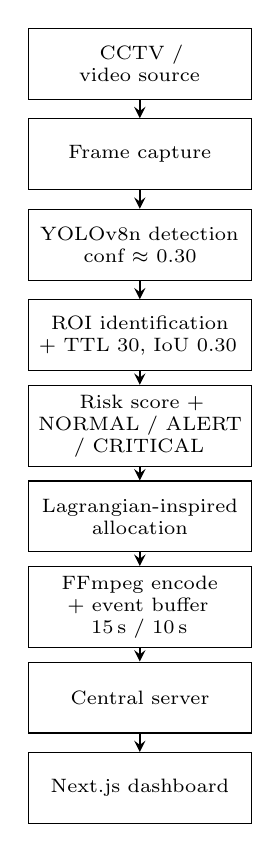
\begin{tikzpicture}[
  node distance=1.15cm, auto,
  block/.style={rectangle, draw, text width=2.6cm, minimum height=0.9cm, align=center, font=\scriptsize},
  arrow/.style={->, >=stealth, thick}
]
\node[block] (src) {CCTV / video source};
\node[block, below of=src] (cap) {Frame capture};
\node[block, below of=cap] (det) {YOLOv8n detection conf $\approx$ 0.30};
\node[block, below of=det] (roi) {ROI identification + TTL 30, IoU 0.30};
\node[block, below of=roi] (risk) {Risk score + NORMAL / ALERT / CRITICAL};
\node[block, below of=risk] (alloc) {Lagrangian-inspired allocation};
\node[block, below of=alloc] (enc) {FFmpeg encode + event buffer 15\,s / 10\,s};
\node[block, below of=enc] (srv) {Central server};
\node[block, below of=srv] (dash) {Next.js dashboard};
\draw[arrow] (src) -- (cap);
\draw[arrow] (cap) -- (det);
\draw[arrow] (det) -- (roi);
\draw[arrow] (roi) -- (risk);
\draw[arrow] (risk) -- (alloc);
\draw[arrow] (alloc) -- (enc);
\draw[arrow] (enc) -- (srv);
\draw[arrow] (srv) -- (dash);
\end{tikzpicture}
\caption{Conceptual pipeline of the implemented system. Each block corresponds to verified code; parameters shown are the evaluated values.}
\label{fig:pipeline}
\end{figure}

[FIGURE PLACEHOLDER --- Figure~1.1 in List of Figures terms: Proposed System Architecture diagram (Edge Node $\rightarrow$ YOLOv8n $\rightarrow$ ROI generation $\rightarrow$ adaptive compression $\rightarrow$ transmission $\rightarrow$ Central Server $\rightarrow$ Dashboard). What to show: deployment-level boxes with data rates and protocols. Purpose: deployment view complementing the pipeline above. Placement: Chapter~5, Section~5.1. Suggested size: 80--90\% of text width. Source: project implementation. Status: NEW FIGURE REQUIRED --- CREATE BEFORE FINAL PRINTING.]

\section{Object Detection and ROI Construction}

Detection uses YOLOv8n (\texttt{edge-node/detector.py}, class \texttt{YoloDetector}, default confidence 0.25 at the API level; 0.30 in all evaluation phases). Detected classes are mapped to priorities by \texttt{priority\_for\_class}: COCO class 0 (person) $\rightarrow$ HIGH; vehicle classes $\{2,3,5,6,7\}$ $\rightarrow$ MEDIUM; all other classes and background $\rightarrow$ LOW. Raw boxes are merged across frames by \texttt{merge\_rois} with IoU threshold 0.30 and smoothing factor 0.4, and each ROI is refreshed with a time-to-live of approximately 30 frames, providing temporal persistence through brief detection gaps. In the Phase~4 comparison, a shared YOLO box cache with 8-pixel dilation was used so that every method operated on identical ROI geometry. Detection is executed on every third frame (\texttt{DETECT\_EVERY\_N} = 3) with CLAHE pre-enhancement when the frame mean falls below 80, and a frame-difference motion fallback fires when no ROI exists but scene change exceeds 0.10.

\section{Risk Scoring and State Assessment}

The heuristic risk score (\texttt{risk\_score} in \texttt{edge-node/capture\_stream.py}) is a weighted sum, capped at 1.0:

\begin{equation}
\mathrm{risk} = \min(1.0,\; 0.30\,n_{\mathrm{HIGH}} + 0.10\,n_{\mathrm{MED}} + 0.03\,n_{\mathrm{LOW}} + 0.25\,\mathrm{motion} + 0.20\,\mathrm{night} + 0.15\,\mathrm{scene} + \min(0.04\,n,\,0.15))
\label{eq:risk}
\end{equation}

where $n_{\mathrm{HIGH}}$, $n_{\mathrm{MED}}$, $n_{\mathrm{LOW}}$ are ROI counts by priority, motion is the normalized frame-difference magnitude, night is a binary indicator (hour $<6$ or $\geq 22$), scene is the scene-change magnitude, and the final term is a density bonus capped at 0.15. The risk score is \textit{primarily a measure of detected-object/ROI importance}; it is not an anomaly probability, and Chapter~7 explains why it must not be read as one. The score drives a three-state machine with hysteresis: risk $\geq$ 0.65 enters CRITICAL; risk $\geq$ 0.30 enters ALERT; CRITICAL exits only below 0.50. States govern compression strength, resolution (640$\times$480 / 854$\times$480 / 1920$\times$1080), GOP structure (120/60, 30/15, 10/5 per state path in the codec manager), and adaptive frame rates.

\section{Lagrangian-Inspired Resource Allocation}

The allocator (\texttt{evaluation/rate\_allocator.py}) distributes a bitrate budget between ROI and background regions. Conceptually, it maximizes a weighted sum of region utilities subject to a total-rate constraint, introducing a Lagrange multiplier $\lambda$ so that each region receives rate $R_i$ satisfying $\partial U_i / \partial R_i = \lambda$; priority weights (HIGH 1.0, MEDIUM 0.4, LOW 0.1) and state-dependent ROI/background budget splits (30/70 NORMAL, 55/45 ALERT, 80/20 CRITICAL) encode ROI importance, and per-ROI rates are clamped to [50, 60\% of ROI budget]. In implementation this is a heuristic solved by a 50-iteration bisection search on $\lambda \in [10^{-6}, 100]$ with tolerance 1.0, using exponential rate--utility models and complexity-adjusted background quality. This thesis therefore describes the method strictly as \textit{Lagrangian-inspired heuristic resource allocation} (a practical approximation), and claims no formally proven global optimality, no convergence guarantee, and no certified optimal bitrate savings. That vocabulary is used consistently throughout the book.

\section{Event Buffering and Forensic Chain}

On entering CRITICAL, the edge node preserves a 15-second pre-event buffer (a frame deque at the operating frame rate) and records a 10-second post-event buffer, dumping frames as JPEG images with per-frame JSON sidecars. After the post-event window completes, \texttt{evaluation/forensic\_chain.py} writes a SHA-256 hash-chained manifest in which each entry links to the previous digest (genesis \texttt{GENESIS}). Verification recomputes digests and chain links over the stored files. The guarantee tested in this thesis is exact-byte integrity behaviour only: recompression, deletion, pixel modification, and sidecar edits are expected to break verification, while untouched evidence is expected to pass. No claim of legal admissibility, certification, or standards compliance is made.

\section{Central Server and Dashboard}

The central server (Node.js/Express with Socket.IO terabits, UDP ingest per camera) relays streams, computes live metrics on a 3-second cadence with automatic bandwidth adaptation, maintains decaying heatmaps, and exposes endpoints for events, motion, cameras, recordings, playback, reconstruction, and 15-second sample requests with real PSNR/SSIM computation. The Next.js dashboard provides live, metrics, playback, and grid views with privacy-mode controls (background blur, face masking, ethical frame-dropping). Details are given in Chapters~5, 6, and 8.

\section{Evaluation Protocols}

\subsection{Phase 1: Public-Dataset Probing}

Protocol (\texttt{evaluation/phase1\_public\_eval.py}): YOLOv8n at confidence 0.30 and 640-pixel width; every 30th frame; frozen risk score; hour fixed to 14 for comparability; CDnet motion threshold 0.0005. CDnet-2014 scenes: \texttt{baseline/highway}, \texttt{baseline/pedestrians}, \texttt{baseline/streetCornerAtNight}. UCF-Crime videos: Normal\_015 and Normal\_050 (normal), Fighting002 (abnormal at clip level; training-split video absent from the supplied annotation pack, so no frame-level evaluation). Burglary001 was excluded because its canonical file could not be verified in isolation; it is documented as not evaluated. Metrics: per-scene risk mean/standard deviation, detection rate, and agreement between detection presence and ground-truth motion inside the temporal ROI; 514 sampled inferences with 0 skipped/failed.

\subsection{Phase 2: Group-Aware Calibration}

Protocol (\texttt{evaluation/phase2\_calibration.py}): 64 labelled seconds (17 positive, 47 negative) from three thesis clips (\texttt{day\_person}, \texttt{day\_empty}, \texttt{night}); labels manually/visually verified with YOLO as assistance only (one night false positive at second 12, a traffic cone, corrected). Model: $P(y{=}1)=\mathrm{sigmoid}(a+b\cdot\mathrm{risk})$ on frozen per-second mean risk, fit with deterministic LBFGS. Splitting: Leave-One-Video-Out (three folds: test on \texttt{day\_empty}, test on \texttt{night}, test on \texttt{day\_person}), plus a full-set descriptive fit. Because all positives come from one video, two test folds are single-class (AUC undefined by construction) and the third train fold is degenerate (zero positives, no fit possible); full-set metrics are therefore apparent/descriptive (in-sample) by construction.

\subsection{Phase 3: Forensic Integrity}

Protocol (\texttt{evaluation/phase3\_forensics.py}): source \texttt{data/thesis\_clips/motion\_only.mp4} (235 frames, 720p); JPEG extraction at quality 2 with JSON sidecars and SHA-256 chain. Five cases with pre-registered expectations: original (expect PASS), clean control (expect PASS), recompressed-vs-original with libx264 CRF 23 (expect FAIL---exact-byte hashes are fragile to transcoding, so this FAIL is a predicted bound, not an experiment failure), recompressed-own-manifest (expect PASS), tampered-vs-pristine with blackout boxes on frames 50/100/150, deletion of \texttt{ev\_00200.jpg}, and sidecar edit of \texttt{ev\_00100\_meta.json} (expect FAIL with localization). Metrics: files checked, missing, hash mismatches, chain mismatches, first failure, localization precision/recall, and clean-case false alarms.

\subsection{Phase 4: Locked Baseline Comparison}

Protocol (\texttt{evaluation/phase4\_sota.py}): primary clip \texttt{motion\_only.mp4} (720p, 235 frames); control clip \texttt{day\_empty.mp4} (777 frames, no ROI); four methods (A uniform, B ROI-QP, C foreground/background split with frozen frame-0 background at 0.5$\times$, D proposed adaptive ROI); bitrate targets 300/600/1200/2400 kbps primary and 300/1200 kbps control; identical source, resolution, frame count, GOP 60 (keyint minimum 30), medium preset, libx265 throughout; one shared YOLOv8n pass per source frame at confidence 0.30 cached to JSON, with 8-pixel dilation and union masks computed from source boxes only (never from encoder outputs); risk thresholds 0.30/0.65 without hysteresis (documented deviation from the live system); background scales 0.25 (B), 0.35/0.60/1.00 by state (D). Metrics: actual bitrate, PSNR/SSIM globally and over ROI/background masks, and detector consistency (recount with the same YOLO on outputs---an internal-consistency check, not independent detection accuracy). BD-rate is reported only if at least four overlapping points, at least 1\,dB of shared interval, and clean fits hold for all comparisons; otherwise it is withheld. Runtime was approximately 3.5 hours wall-clock (9764\,s) on the CPU-only machine.


% Create Chapter 5: System Architecture and Design
\chapter{SYSTEM ARCHITECTURE DESIGN}
% Insert System Architecture and Design chapter content from external file
\section{System Overview}

The system follows an edge-cloud style architecture with three tiers: the Edge Node, the Central Server, and the Next.js dashboard. The Edge Node performs capture, detection, ROI generation, risk assessment, adaptive encoding, and event buffering. The Central Server ingests streams from multiple cameras, maintains metrics and heatmaps, manages recordings and playback, and serves the dashboard. The dashboard provides live viewing, metric visualization, forensic playback, and privacy controls. This decomposition keeps bandwidth-intensive pixel processing at the edge while centralizing state, storage, and user interaction, consistent with established edge-cloud surveillance designs \cite{Chen2019DIVS,Elgamal2020SIEVE,Nan2023Collaborative}.

[FIGURE PLACEHOLDER --- Figure~5.1: Overall architecture of the proposed adaptive CCTV compression system (deployment view). What to show: Edge Node box (capture, YOLOv8n, ROI, risk, FFmpeg, event buffer) $\rightarrow$ network (UDP/Socket.IO) $\rightarrow$ Central Server box (ingest, metrics, heatmap, recordings, forensic verify) $\rightarrow$ Next.js dashboard box (live, metrics, playback, grid). Purpose: deployment-level visual complement to the pipeline in Figure~4.1. Placement: immediately after this section. Suggested size: 80--90\% of text width. Source: project implementation. Status: NEW FIGURE REQUIRED --- CREATE BEFORE FINAL PRINTING, following the TikZ style of Figure~4.1.]

\section{Edge Node Architecture}

The Edge Node is a Python service built around \texttt{edge-node/capture\_stream.py} with detection abstracted in \texttt{edge-node/detector.py}. Its internal data flow is: camera frame $\rightarrow$ optional CLAHE enhancement $\rightarrow$ YOLOv8n inference (every third frame) $\rightarrow$ ROI merge with 30-frame TTL $\rightarrow$ motion/scene estimation $\rightarrow$ risk scoring (Equation~\ref{eq:risk}) $\rightarrow$ state machine with hysteresis $\rightarrow$ allocation (heuristic path via state-compression table or optimizer path via \texttt{RateAllocator}) $\rightarrow$ FFmpeg encoding with per-state GOP, resolution, and bitrate $\rightarrow$ UDP/Socket.IO transmission plus local event-buffer dumps. Supporting modules include the camera manager, PTZ controller, ReID tracker, audio monitor, and YAMNet classifier, which are present in the repository but outside the evaluated compression path and therefore documented here without evaluation claims.

\section{Risk-State Machine}

\begin{figure}[H]
\centering
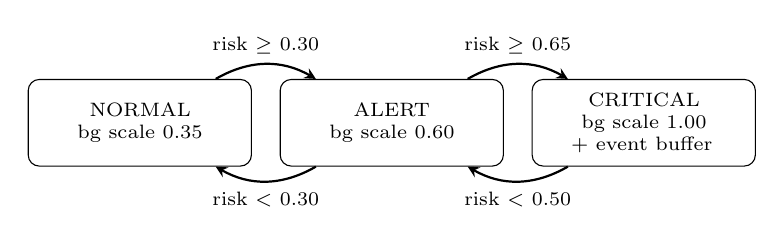
\begin{tikzpicture}[
  node distance=3.2cm, auto,
  state/.style={rectangle, draw, rounded corners, text width=2.6cm, minimum height=1.1cm, align=center, font=\scriptsize},
  arrow/.style={->, >=stealth, thick, font=\scriptsize}
]
\node[state] (n) {NORMAL \\ bg scale 0.35};
\node[state, right of=n] (a) {ALERT \\ bg scale 0.60};
\node[state, right of=a] (c) {CRITICAL \\ bg scale 1.00 + event buffer};
\draw[arrow] (n) to[bend left] node[above] {risk $\geq$ 0.30} (a);
\draw[arrow] (a) to[bend left] node[above] {risk $\geq$ 0.65} (c);
\draw[arrow] (c) to[bend left] node[below] {risk $<$ 0.50} (a);
\draw[arrow] (a) to[bend left] node[below] {risk $<$ 0.30} (n);
\end{tikzpicture}
\caption{Risk-state machine with hysteresis. CRITICAL additionally triggers 15\,s pre-event and 10\,s post-event buffering with forensic manifests.}
\label{fig:state-machine}
\end{figure}

The state machine uses hysteresis (CRITICAL exit at 0.50 versus entry at 0.65) to prevent oscillation at boundaries, with an 8-frame smoothing hysteresis in the live path. State transitions reconfigure GOP length, resolution, compression strength, and frame rate, and CRITICAL additionally opens an event record with server notification.

\section{Central Server Architecture}

The Central Server (\texttt{server/server.js}) is an Express/Socket.IO application accepting per-camera UDP streams. It computes stream metrics every 3000\,ms with automatic bandwidth adaptation (background quality/scale/floor adjusted when measured throughput exceeds twice the 128\,kbps threshold), maintains heatmaps with 300-second decay capped at 10000 points weighted by ROI priority, and exposes REST/Socket endpoints for events, motion, heatmaps, cameras, recordings, playback, reconstruction, and 15-second sample requests with real PSNR/SSIM computation. Recordings are retained on a 7-day hourly rotation. Adaptive streaming rules with exponential moving averaging (factor 0.3), 5-second cooldown, and user-override locking are implemented but disabled by default; this thesis makes no performance claim about them.

\section{Dashboard Architecture}

The dashboard (\texttt{dashboard/src/app}) is a Next.js application with \texttt{live/}, \texttt{metrics/}, \texttt{playback/}, and \texttt{grid/} views plus shared components, configuration, and library layers. It renders live streams, metric time series, heatmap overlays, forensic playback with manifest status, and multi-camera grids, and exposes privacy-mode controls. Screenshots are reserved in Chapter~8.

\section{Configuration Profiles}

Four YAML deployment profiles parameterize the system: \texttt{balanced} (1280$\times$720, 10/20\,fps, hevc\_nvenc p4, 800\,kbps, confidence 0.5), \texttt{high\_quality} (1920$\times$1080, 24/30\,fps, 2000\,kbps, confidence 0.6), \texttt{ultra\_low\_bandwidth} (640$\times$480, 5/10\,fps, 200\,kbps, confidence 0.4), and \texttt{privacy\_mode} (1280$\times$720, 5/15\,fps, 500\,kbps with background blur, face masking, and ethical frame-dropping). Evaluation phases used their own frozen parameters (confidence 0.30, documented per phase) rather than these deployment presets, and the two regimes are not mixed in any reported number.

\begin{table}[H]
\centering
\caption{Deployment configuration profiles (\texttt{configs/*.yaml})}
\label{tab:profiles}
\begin{tabular}{|l|c|c|c|c|}
\hline
\textbf{Profile} & \textbf{Resolution} & \textbf{Bitrate} & \textbf{Conf.} & \textbf{Privacy} \\
\hline
balanced & 1280$\times$720 & 800\,kbps & 0.5 & blur 51 \\
high\_quality & 1920$\times$1080 & 2000\,kbps & 0.6 & off \\
ultra\_low\_bandwidth & 640$\times$480 & 200\,kbps & 0.4 & blur 99 \\
privacy\_mode & 1280$\times$720 & 500\,kbps & 0.5 & blur 99 + mask + ethical drop \\
\hline
\end{tabular}
\end{table}


% Create Chapter 6: System Implementaion
\chapter{SYSTEM IMPLEMENTATION}
% Insert System implementation
\section{Edge Node Implementation}

The edge implementation centers on two files. \texttt{edge-node/detector.py} provides a pluggable detector registry (\texttt{yolo}, \texttt{mock}) with \texttt{YoloDetector} wrapping the YOLOv8n weights and a class-to-priority map (person HIGH; vehicle classes $\{2,3,5,6,7\}$ MEDIUM; remainder LOW). \texttt{edge-node/capture\_stream.py} implements the \texttt{AdaptiveRateAllocator}, the \texttt{CodecManager} (GOP and resolution ladders), the \texttt{reconstruct} path (ethical black frames when no ROI exists under ethical mode; background blur with kernel (99,99); background down/up-scaling; 0.7$\times$ medium-region recompression; face blurring for HIGH regions under masking), ROI merging (IoU 0.30, smoothing 0.4, TTL refresh), the risk score of Equation~\ref{eq:risk}, the hysteresis state machine, and the preview path (JPEG quality 82, heatmap refresh every 5 frames with 15-frame persistence, motion estimation cadence \texttt{DETECT\_EVERY\_N} = 3). Adaptive frame-rate reduction (halving down to a floor of 5\,fps when NORMAL with no ROI) and the confidence split (0.20 in low light, else 0.30) are implemented as described; neither is credited with a measured performance gain in this thesis.

\section{Compression and Allocation Implementation}

Two allocation paths exist. The heuristic path applies the state-compression table (NORMAL: no override; ALERT: 0.75 scale / quality 45/95; CRITICAL: 1.0 scale / quality 88/100). The optimizer path calls \texttt{evaluation/rate\_allocator.py::RateAllocator} with priority weights 1.0/0.4/0.1, complexity-aware background quality, track-boosted importance ($\times$1.3), per-ROI clamping, and the 50-iteration $\lambda$ bisection described in Chapter~4. FFmpeg invocation uses fast presets for libx265/libx264, p1 for NVENC, preset 8 with CRF 35 for SVT-AV1, and realtime/cpu-used 8 for VP9, with bitrate, 1.5$\times$ maxrate, 2$\times$ bufsize, and GOP-derived keyframe intervals. The Phase~4 encodes used libx265 medium with GOP 60 and keyint minimum 30 through a raw-video pipe (single-encode by construction, no intermediate file).

\section{Event Buffering and Forensic Implementation}

On the NORMAL$\rightarrow$ALERT$\rightarrow$CRITICAL escalation, the edge node opens an \texttt{event\_\textless ms\textgreater} record, flushes the 15-second pre-event deque (frames plus metadata JSON) to disk, notifies the server via POST /event, and accumulates the 10-second post-event window before calling \texttt{forensic\_chain.write\_manifest}. The manifest format stores per-file SHA-256 digests with backward chain links from a \texttt{GENESIS} anchor over the sorted set of \texttt{pre\_*.jpg}, \texttt{pre\_*\_meta.json}, and \texttt{post\_*.jpg} files. Verification (\texttt{verify\_all} in the Phase~3 harness) checks every file and reports missing files, direct hash mismatches, downstream chain breaks, and the first failure; it is intentionally exhaustive rather than early-stopping so that tamper localization can be scored.

\section{Server and Dashboard Implementation}

The server implementation follows the architecture of Chapter~5: UDP ingest, 3-second metric cadence, threshold-triggered bandwidth adaptation, decaying heatmaps, and the endpoint set for events, motion, cameras, recordings, playback, reconstruction, and sample requests. The dashboard implements the four views with shared component and library layers. Both tiers were exercised during development; systematic quantitative evaluation of server/dashboard performance (latency, throughput, concurrent users) was not performed and is recorded as not available in the current evidence rather than estimated.

\section{Algorithm Summary}

\begin{table}[H]
\centering
\caption{Key implementation parameters (evaluated values)}
\label{tab:params}
\begin{tabular}{|l|l|}
\hline
\textbf{Parameter} & \textbf{Value} \\
\hline
Detector & YOLOv8n, confidence $\approx$ 0.30 (evaluation) \\
ROI policy & person HIGH / vehicle MEDIUM / other LOW \\
ROI merge & IoU 0.30, smoothing 0.4, TTL $\approx$ 30 frames \\
Phase~4 dilation & 8 px, shared box cache, union masks \\
Risk thresholds & 0.30 ALERT / 0.65 CRITICAL / 0.50 CRITICAL-exit \\
Event buffer & 15\,s pre-event / 10\,s post-event \\
GOP / keyint (Phase~4) & 60 / 30, libx265 medium \\
Bitrate targets (Phase~4) & 300 / 600 / 1200 / 2400 kbps \\
Codec fairness & same source, resolution, frames, GOP, codec \\
Hardware & CPU-only (i3-6006U, 4 logical CPUs, no GPU) \\
\hline
\end{tabular}
\end{table}

[FIGURE PLACEHOLDER --- Figure~6.1: YOLO detection with ROI overlay example on a thesis clip frame. What to show: one annotated frame with HIGH/MEDIUM/LOW boxes and the risk/state readout. Purpose: to ground the ROI policy in a concrete visual. Placement: after Section~6.1. Suggested size: 70--80\% of text width. Source: project implementation (generate from \texttt{day\_person.mp4} with the preview path). Status: NEW FIGURE REQUIRED --- CREATE BEFORE FINAL PRINTING.]


% Create Chapter 7: Result and Discussion
\chapter{RESULT \& DISCUSSION}
% Insert Result and Discussion chapter content from external file
\section{Overview of Experiments}

Four evaluation phases were executed against frozen code with provenance recording (git commit \texttt{7e08016}, CPU-only Intel i3-6006U, no GPU). Phase~1 probed public datasets (CDnet-2014, UCF-Crime; 514 sampled inferences, 0 skipped/failed, 88.7\,s). Phase~2 calibrated the risk score over 64 labelled seconds (473 inferences, 176.1\,s) under Leave-One-Video-Out. Phase~3 tested forensic integrity over 470 frames per case. Phase~4 ran the locked baseline comparison (24 encodes: 16 primary + 8 control; $\approx$ 3.5 hours wall-clock, 9764\,s). This chapter reports each phase in RESULT $\rightarrow$ EVIDENCE $\rightarrow$ INTERPRETATION $\rightarrow$ LIMITATION order. Numbers below are taken verbatim from \texttt{experiments/phase{1,2,3,4}\_*/} CSV and JSON evidence files.

\section{Phase 1: Public-Dataset Observations}

\subsection{CDnet-2014}

\begin{table}[H]
\centering
\caption{Phase~1 CDnet-2014 results (confidence 0.30, every 30th frame, hour fixed to 14)}
\label{tab:phase1-cdnet}
\begin{tabular}{|l|c|c|c|c|c|}
\hline
\textbf{Scene} & \textbf{Samples} & \textbf{Risk mean $\pm$ std} & \textbf{Detect.\ rate} & \textbf{Agreement} & \textbf{TP/FP/FN} \\
\hline
highway & 57 (41 in ROI) & 0.563 $\pm$ 0.234 & 0.983 & 0.976 & 40/0/1 \\
pedestrians & 37 (27 in ROI) & 0.492 $\pm$ 0.264 & 1.000 & 0.778 & 21/6/0 \\
streetCornerAtNight & 174 (147 in ROI) & 0.024 $\pm$ 0.056 & 0.121 & 0.803 & 10/8/21\footnotemark \\
\hline
\end{tabular}
\end{table}
\footnotetext{TN = 108 for streetCornerAtNight; TN = 0 for highway and pedestrians (temporal ROI contains motion throughout).}

RESULT: On highway, the risk score averaged $0.563 \pm 0.234$ with agreement 0.976 (40 TP, 0 FP, 1 FN). EVIDENCE: \texttt{experiments/phase1\_public/cdnet\_scene\_results.csv}. INTERPRETATION: where persistent person/vehicle activity fills the temporal ROI, detection presence aligns closely with ground-truth motion and the risk score sits in the ALERT band. LIMITATION: the temporal ROI of this scene contains almost no negative samples (TN = 0), so agreement here measures recall-like behaviour, not balanced accuracy; the hour was fixed to 14 for comparability, which is artificial for the night scene.

RESULT: On pedestrians, risk averaged $0.492 \pm 0.264$ with agreement 0.778 (21 TP, 6 FP, 0 FN). INTERPRETATION: the detector fires reliably (detection rate 1.0) but produces false positives relative to the motion ground truth, consistent with a detector-presence signal that is broader than pixel-motion truth. LIMITATION: same single-class-positive caveat as highway.

RESULT: On streetCornerAtNight, risk averaged $0.024 \pm 0.056$ with detection rate 0.121 and agreement 0.803 (10 TP, 108 TN, 8 FP, 21 FN). INTERPRETATION: under night conditions with the hour artificially fixed to 14 (no night bonus) and CPU-only YOLOv8n at 640-pixel width, the detector largely misses the scene's motion content; the high TN count sustains agreement despite 21 false negatives. LIMITATION: this scene exposes the detector's night weakness and the hour-fixing limitation simultaneously; it must not be read as a general night-performance claim.

\subsection{UCF-Crime}

\begin{table}[H]
\centering
\caption{Phase~1 UCF-Crime results (clip-level labels; Fighting002 training-split, annotation pack absent)}
\label{tab:phase1-ucf}
\begin{tabular}{|l|c|c|c|c|}
\hline
\textbf{Video} & \textbf{Label} & \textbf{Risk mean $\pm$ std} & \textbf{Detect.\ rate} & \textbf{Samples} \\
\hline
Normal\_015 & normal & 0.467 $\pm$ 0.360 & 0.938 & 16 \\
Normal\_050 & normal & 0.994 $\pm$ 0.033 & 1.000 & 140 \\
Fighting002 & abnormal & 0.068 $\pm$ 0.135 & 0.311 & 90 \\
\hline
\end{tabular}
\end{table}

RESULT: Normal\_050 (normal label) scored risk $\approx$ 0.994 while Fighting002 (abnormal label) scored risk $\approx$ 0.068 with detection rate 0.311. EVIDENCE: \texttt{experiments/phase1\_public/ucf\_video\_results.csv} and \texttt{annotation\_check.json}. INTERPRETATION: this inversion is expected once the two quantities are correctly understood---the heuristic risk score measures detected-object/ROI importance (crowded normal scenes score highly), whereas UCF-Crime anomaly labels annotate video-level abnormal events (a distant fight with few confident detections scores lowly). High risk therefore does \textit{not} mean anomaly, and the two concepts are not equivalent. LIMITATION: Fighting002 comes from the training split with the annotation pack unavailable, so only the clip-level label was used and no frame-level ground-truth evaluation is claimed; Burglary001 was not evaluated at all because its canonical file could not be verified in isolation.

\section{Phase 2: Calibration Analysis}

\subsection{Label Basis}

The calibration set comprises 64 seconds (17 positive, 47 negative) from \texttt{day\_person}, \texttt{day\_empty}, and \texttt{night} (\texttt{evaluation/labels/*.csv}), manually/visually verified with YOLO as assistance only; one night false positive at second 12 (a traffic cone) was corrected. All 17 positives originate from a single video (\texttt{day\_person}). The fitted model is $P(y{=}1)=\mathrm{sigmoid}(a+b\cdot\mathrm{risk})$ on frozen per-second mean risk.

\subsection{Leave-One-Video-Out Behaviour}

\begin{table}[H]
\centering
\caption{Phase~2 Leave-One-Video-Out folds (AUC undefined for single-class tests by construction)}
\label{tab:phase2-lovo}
\begin{tabular}{|l|l|c|c|c|}
\hline
\textbf{Fold} & \textbf{Test clip} & \textbf{n train/test} & \textbf{Outcome} & \textbf{Brier} \\
\hline
F1 & day\_empty (all negative) & 38 / 26 & specificity only, no AUC & 0.0536 \\
F2 & night (all negative) & 43 / 21 & specificity only, no AUC & 0.1422 \\
F3 & day\_person (all positive) & 47 / 17 & degenerate: 0-positive train, no fit & --- \\
FULL & all (descriptive) & 64 / 64 & apparent metrics only & 0.0878 \\
\hline
\end{tabular}
\end{table}

RESULT: F1 and F2 test folds are single-class (all negative), so ROC-AUC is mathematically undefined and was not reported; F1 achieved specificity 1.0 (26/26 TN) while F2 showed 18 false positives against 3 true negatives at its fitted threshold. F3 could not be fit at all because its training set contained zero positives. EVIDENCE: \texttt{experiments/phase2\_calibration/calibration\_results.json}, \texttt{calibration\_metrics.csv}. INTERPRETATION: the label distribution (positives concentrated in one video) makes independent generalization untestable under LOVO; the folds diagnose the data limitation rather than the model. LIMITATION: no fold constitutes an independent generalization test.

\subsection{Full-Set Descriptive Metrics}

RESULT: The full-set descriptive fit ($a=-2.0055$, $b=3.4353$, threshold 0.35) yields AUC $\approx$ 0.9962, F1 $\approx$ 0.919, precision $\approx$ 0.850, recall = 1.00, specificity $\approx$ 0.936, PR-AUC $\approx$ 0.990, and Brier $\approx$ 0.088 (baseline frozen-risk at 0.30: F1 0.850, Brier 0.064). EVIDENCE: \texttt{calibration\_metrics.csv}, \texttt{coefficients.csv}, \texttt{threshold\_grid.csv}. INTERPRETATION: within-sample, per-second mean risk separates the 64 labelled seconds well, and the fitted logistic improves over the frozen 0.30 threshold on F1. LIMITATION: these metrics are apparent/descriptive/in-sample by construction---they reuse the training data as the test data and all positives come from one video---so they establish separability of this small labelled set only, and must never be headlined as 99.6\% AUC, 100\% recall, or perfect detection without that qualification.

\begin{figure}[H]
\centering
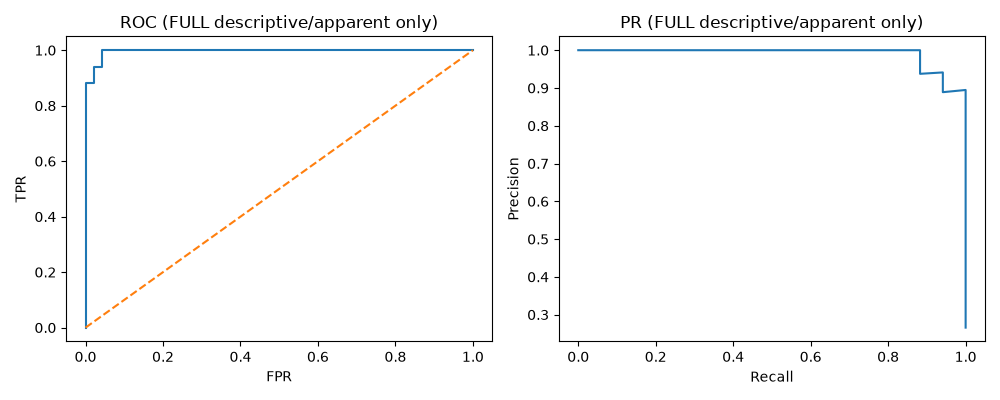
\includegraphics[width=0.85\textwidth]{figures/phase2_roc_pr.png}
\caption{Phase~2 full-set apparent ROC and precision--recall curves (in-sample, descriptive only; not generalization evidence). Source: \texttt{experiments/phase2\_calibration/roc\_pr\_full\_apparent.png}.}
\label{fig:phase2-roc}
\end{figure}

\begin{figure}[H]
\centering
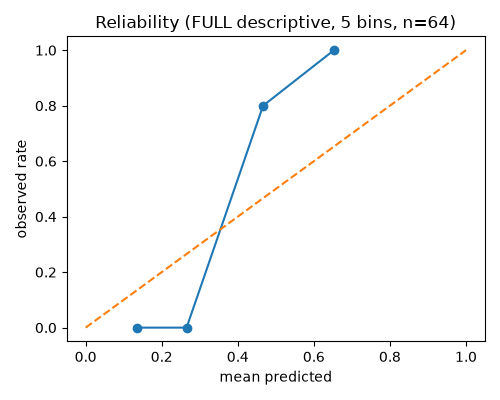
\includegraphics[width=0.85\textwidth]{figures/phase2_reliability.png}
\caption{Phase~2 reliability diagram for the full-set descriptive fit ($n=64$). Source: \texttt{experiments/phase2\_calibration/reliability\_full.png}.}
\label{fig:phase2-rel}
\end{figure}

\section{Phase 3: Forensic Integrity}

\begin{table}[H]
\centering
\caption{Phase~3 forensic cases (470 frames; source \texttt{data/thesis\_clips/motion\_only.mp4})}
\label{tab:phase3}
\begin{tabular}{|l|c|c|c|c|}
\hline
\textbf{Case} & \textbf{Expected} & \textbf{Verdict} & \textbf{Detail} & \textbf{Met} \\
\hline
original & PASS & PASS & 470/470 pass & Yes \\
clean\_control & PASS & PASS & 470/470 pass & Yes \\
recompressed\_vs\_original & FAIL & FAIL & 470/470 mismatch from ev\_00001.jpg & Yes \\
recompressed\_own\_manifest & PASS & PASS & 470/470 pass & Yes \\
tampered\_vs\_pristine & FAIL & FAIL & 1 missing, 4 hash, 416 chain; first ev\_00050.jpg & Yes \\
\hline
\end{tabular}
\end{table}

RESULT: All five cases met their pre-registered expectations. Direct tamper localization scored 5/5 detected (precision 1.0, recall 1.0) with zero false alarms in clean cases. EVIDENCE: \texttt{experiments/phase3\_forensics/cases.csv}, \texttt{localization.csv}, \texttt{custody.json}. INTERPRETATION: the hash chain behaves as an exact-byte tamper-evident mechanism---it passes untouched evidence (including a freshly generated manifest over recompressed content) and fails loudly on any byte-level alteration, with cascade breaks that localize the first tamper point. The recompression FAIL is a predicted bound of exact-byte hashing, not an experiment failure. LIMITATION: this demonstrates exact-byte/hash-chain integrity behaviour only; it establishes no legal admissibility, court-grade validity, certification, standards compliance, or real-world chain-of-custody sufficiency, and only the listed tampering operations were tested.

\begin{figure}[H]
\centering
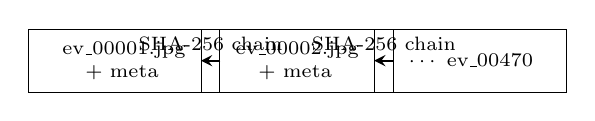
\begin{tikzpicture}[
  node distance=2.2cm, auto,
  file/.style={rectangle, draw, text width=2.2cm, minimum height=0.8cm, align=center, font=\scriptsize},
  arrow/.style={->, >=stealth, thick, font=\scriptsize}
]
\node[file] (f1) {ev\_00001.jpg + meta};
\node[file, right of=f1] (f2) {ev\_00002.jpg + meta};
\node[file, right of=f2] (f3) {$\cdots$ ev\_00470};
\draw[arrow] (f1) -- node[above] {SHA-256 chain} (f2);
\draw[arrow] (f2) -- node[above] {SHA-256 chain} (f3);
\end{tikzpicture}
\caption{Tamper-evident hash-chain structure: each manifest entry binds the file digest to the previous link from a GENESIS anchor. Any deletion, pixel edit, or sidecar modification breaks its own link and every downstream link.}
\label{fig:hashchain}
\end{figure}

[FIGURE PLACEHOLDER --- Figure~7.5: Tampering example (blackout box on frames 50/100/150). What to show: one tampered frame with the (500,200,200,200) blackout region marked. Purpose: concrete illustration of the tested tamper operations. Placement: after Section~7.3. Suggested size: 60--70\% of text width. Source: \texttt{experiments/phase3\_forensics/evidence\_tampered/}. Status: AVAILABLE --- NEEDS FORMATTING (export single frame with annotation).]

\section{Phase 4: Controlled Baseline Comparison}

\subsection{Rate--Distortion Behaviour}

RESULT: On the primary clip (motion\_only, 720p, 235 frames, libx265), measured operating points were: uniform $\approx$ 495/840/1520/2832 kbps with PSNR $\approx$ 36.5/39.4/42.3/45.2; ROI-QP $\approx$ 360/721/1434/2806 kbps with PSNR $\approx$ 33.5/35.5/37.1/38.4; foreground/background split $\approx$ 382/770/1540/3085 kbps with PSNR $\approx$ 13.4--13.5 flat; proposed adaptive ROI $\approx$ 355/710/1399/2754 kbps with PSNR $\approx$ 33.8/36.2/38.1/39.7. ROI-PSNR ranges were 31.5--41.6 (uniform), 28.8--36.6 (ROI-QP), 20.9--21.5 (split), and 28.7--37.0 (proposed); background PSNR ranges were 38.4--46.4 (uniform), 35.5--39.1 (ROI-QP), $\approx$ 12.8 flat (split), and 35.9--40.8 (proposed). EVIDENCE: \texttt{experiments/phase4\_sota/roi\_metrics.csv}, \texttt{runs.csv}. INTERPRETATION: the ROI-based methods operate at lower bitrates than uniform at the same targets (they discard background information by design) but at lower global and ROI fidelity on this sequence; the foreground/background split's flat $\approx$ 13.5 dB PSNR is a negative result caused by its frozen-frame-0 background assumption being inappropriate for the moving-camera clip. LIMITATION: conclusions are confined to the evaluated configuration (single primary motion clip, CPU libx265 medium, stated background scales).

\begin{figure}[H]
\centering
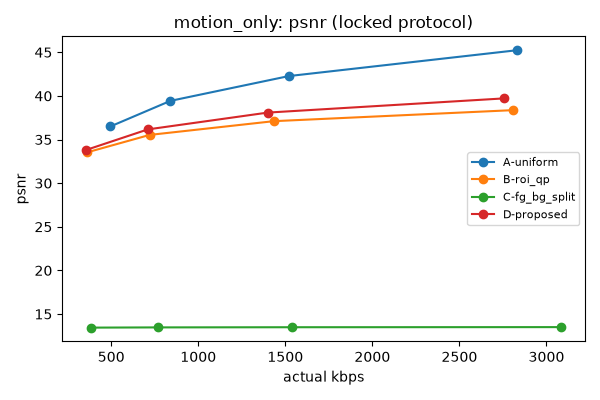
\includegraphics[width=0.85\textwidth]{figures/phase4_rd_psnr.png}
\caption{Phase~4 global rate--distortion curves (PSNR vs.\ actual bitrate, motion\_only, libx265). Source: \texttt{experiments/phase4\_sota/rd\_psnr.png}.}
\label{fig:rd-psnr}
\end{figure}

\begin{figure}[H]
\centering
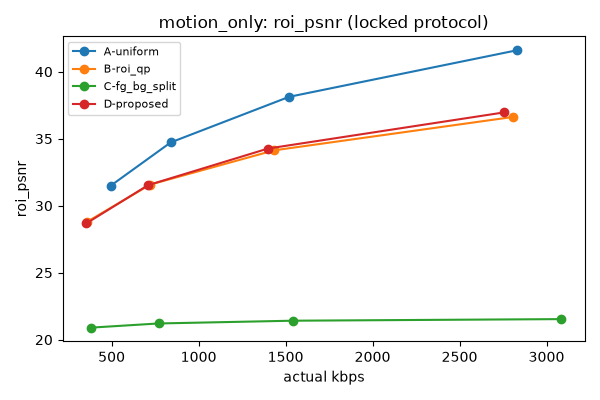
\includegraphics[width=0.85\textwidth]{figures/phase4_rd_roi.png}
\caption{Phase~4 ROI rate--distortion curves (ROI-PSNR vs.\ actual bitrate). Source: \texttt{experiments/phase4\_sota/rd\_roi.png}.}
\label{fig:rd-roi}
\end{figure}

\begin{figure}[H]
\centering
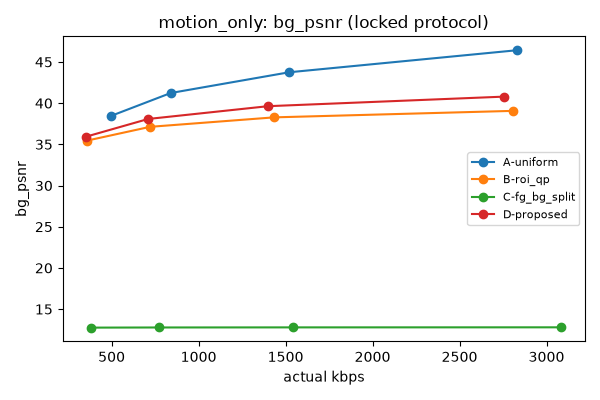
\includegraphics[width=0.85\textwidth]{figures/phase4_rd_bg.png}
\caption{Phase~4 background rate--distortion curves (BG-PSNR vs.\ actual bitrate); note the flat foreground/background-split curve. Source: \texttt{experiments/phase4\_sota/rd\_bg.png}.}
\label{fig:rd-bg}
\end{figure}

\subsection{Matched-Bitrate Comparison (Primary Result)}

\begin{table}[H]
\centering
\caption{Phase~4 matched-bitrate comparison ($\approx$ 710--840 kbps operating region)}
\label{tab:matched}
\begin{tabular}{|l|c|c|c|c|}
\hline
\textbf{Method} & \textbf{Actual kbps} & \textbf{PSNR} & \textbf{ROI-PSNR} & \textbf{BG-PSNR} \\
\hline
A uniform @600 & 839.7 & 39.43 & 34.72 & 41.23 \\
B ROI-QP @600 & 721.2 & 35.53 & 31.57 & 37.13 \\
D proposed @600 & 710.2 & 36.16 & 31.54 & 38.08 \\
\hline
\end{tabular}
\end{table}

RESULT: At the matched bitrate of approximately 710--840 kbps, uniform encoding achieved ROI-PSNR $\approx$ 34.7 dB versus $\approx$ 31.6 dB (ROI-QP) and $\approx$ 31.5 dB (proposed). EVIDENCE: \texttt{experiments/phase4\_sota/matched\_bitrate.csv}. INTERPRETATION: the current ROI construction did \textit{not} demonstrate a quality advantage over uniform encoding at matched bitrate; uniform encoding's even allocation preserved more ROI fidelity per bit on this sequence than the tested background-degrading constructions. A plausible explanation is that the current ROI geometry and background scales do not compensate for the spatial/temporal characteristics of the moving-camera sequence (large ROI coverage of 234/235 frames leaves little background to save on, while the quality penalty on the remainder drags both global and ROI reconstruction). This is a legitimate negative result: it reveals the limits of the current ROI construction rather than the ineffectiveness of ROI-based compression in general, and it is reported without distortion. LIMITATION: single primary clip; no claim about other scenes, codecs, or ROI constructions is made.

\subsection{BD-Rate, Consistency, and Control Clip}

RESULT: BD-rate was withheld (\texttt{reported=false}; \texttt{experiments/phase4\_sota/bd\_diagnostics.json}) because the protocol preconditions (at least four overlapping points, at least 1\,dB of shared interval, clean fits for all comparisons) were not satisfied; the computed-but-suppressed values are not reported as results. Any older -87.95\%/-83.15\% figures found in project logs are superseded single-clip/unaudited values from an earlier regime and are not main results. Detector consistency was 1.0 across all 24 runs; because the same YOLO-generated boxes constructed the ROI and performed the recounting, this is internal pipeline consistency, not independent detection accuracy, and it is labelled accordingly. The no-ROI control clip (day\_empty, 777 frames) behaved as expected: all methods converged toward uniform-like operating points with no ROI to exploit.

\section{Comparison with Literature}

The literature reports substantial ROI-based savings under its own protocols---for example, approximately -32\% versus H.265 at matched quality for ROI-DVC \cite{Wu2024ROIDVC}, approximately -50.4\% with accuracy held for How2Compress \cite{Wu2025How2Compress}, approximately -49.75\% bpp at 36\,dB for foreground-background parallel compression \cite{Wu2020FGBG}, bandwidth reductions of approximately 25.0--76.9\% for VaBUS \cite{Wang2023VaBUS}, and approximately -74.63\% data for semantic-aware offloading \cite{Kadukar2026Semantic}. Those figures were obtained with different scenes (frequently static-camera), codecs, ROI constructions, and quality metrics, and several use learned or GPU-assisted machinery \cite{Wu2024ROIDVC,Zhao2025ASVC,Zhao2025TALC} unlike the CPU-only heuristic tested here. The present negative result therefore does not contradict those studies; it bounds them, showing that an ROI advantage cannot be assumed for moving-camera content under same-codec, shared-cache, matched-bitrate conditions. This is consistent with the scene-dependence already noted for aerial ROI coding \cite{Meuel2018Aerial} and with the codec-independent ROI view that background-degrading constructions must be matched to scene statistics \cite{CodecIndependent2016}.

\section{Limitations of the Evaluation}

The evaluation is limited by: a small calibration set with positives from one video; single-class LOVO folds; hour-fixing in Phase~1; a single primary motion clip in Phase~4; a limited tamper-operation set with exact-byte scope; CPU-only execution; no independent detector ground truth in Phase~4; withheld BD-rate; and the documented deviation of dropped hysteresis in Phase~4 relative to the live system. Old exploratory claims (87.95\% BD-rate reduction, 83.15\%, greater than 95\% recall, 20.4 FPS, 217 kbps, 0.913 SSIM) were traced to earlier experimental regimes and are demoted: they are not reproducible under the final locked protocol and appear nowhere as headline results. Every number in this chapter traces to the cited evidence file; conflicting values between old documents and the final CSV/JSON evidence were resolved in favour of the final evidence.


% Create Chapter 8: Web Application, 
\chapter{WEB APPLICATION}
\section{Overview}

The web application tier comprises the Central Server (Node.js/Express with Socket.IO) and the Next.js dashboard. It provides live multi-camera viewing, metric visualization, forensic playback with manifest status, heatmap overlays, recording management, and privacy-mode controls. This chapter describes the implemented functionality as built; systematic performance evaluation of the server/dashboard tier (latency, throughput, concurrent users) was not performed and is stated as not available in the current evidence.

\section{Central Server Services}

The server ingests one UDP stream per camera (ports configured in \texttt{configs/cameras.yaml}), relays live video over Socket.IO, computes stream metrics on a 3-second cadence with threshold-triggered automatic bandwidth adaptation, and maintains heatmaps with 300-second decay capped at 10000 points weighted HIGH=3/MEDIUM=2/LOW=1. Its endpoint set covers events, motion, heatmaps, cameras, recordings, playback, reconstruction, and 15-second sample requests with real PSNR/SSIM computation. Recordings rotate on a 7-day hourly schedule. Adaptive streaming rules (risk-tiered quality/scale/floor with EMA factor 0.3, 5-second cooldown, 10--15\,s user-override locking) are implemented but disabled by default.

\section{Dashboard Views}

The Next.js dashboard implements four views: \texttt{live/} for real-time streams with ROI overlays and state readouts; \texttt{metrics/} for bitrate, PSNR/SSIM, risk, and state time series; \texttt{playback/} for event-centered forensic review with integrity-manifest status; and \texttt{grid/} for multi-camera walls. Privacy controls expose background blur, face masking, and ethical frame-dropping per the active YAML profile.

[FIGURE PLACEHOLDER --- Figure~8.1: Dashboard live-view screenshot. What to show: live stream with ROI overlays, risk/state readout, and metric panel. Purpose: to document the operator-facing interface. Placement: after Section~8.3. Suggested size: 85--95\% of text width. Source: running dashboard. Status: NEW SCREENSHOT REQUIRED --- CAPTURE BEFORE FINAL PRINTING.]

[FIGURE PLACEHOLDER --- Figure~8.2: Dashboard metrics/playback screenshot. What to show: metric time series and one forensic playback panel with manifest status. Purpose: to document monitoring and forensic-review interfaces. Placement: after Figure~8.1. Suggested size: 85--95\% of text width. Source: running dashboard. Status: NEW SCREENSHOT REQUIRED --- CAPTURE BEFORE FINAL PRINTING.]


% Create Chapter 9: Project and Time Management
\chapter{PROJECT and TIME MANAGEMENT}
% Insert Project and Time Management chapter content from external file
\section{Project and Timeline Management}

\subsection{Completion Timeline}

The project proceeded in five stages: (1) prototype construction (edge node, server, dashboard); (2) public-dataset probing (Phase~1); (3) calibration analysis (Phase~2); (4) forensic-integrity testing (Phase~3); and (5) the locked baseline comparison (Phase~4, $\approx$ 3.5 hours wall-clock on CPU-only hardware). Each experiment directory records its command, timestamp, git commit, and hardware provenance, providing the audit trail used throughout this book.

\subsection{Gantt Chart}

\begin{figure}[H]
\centering
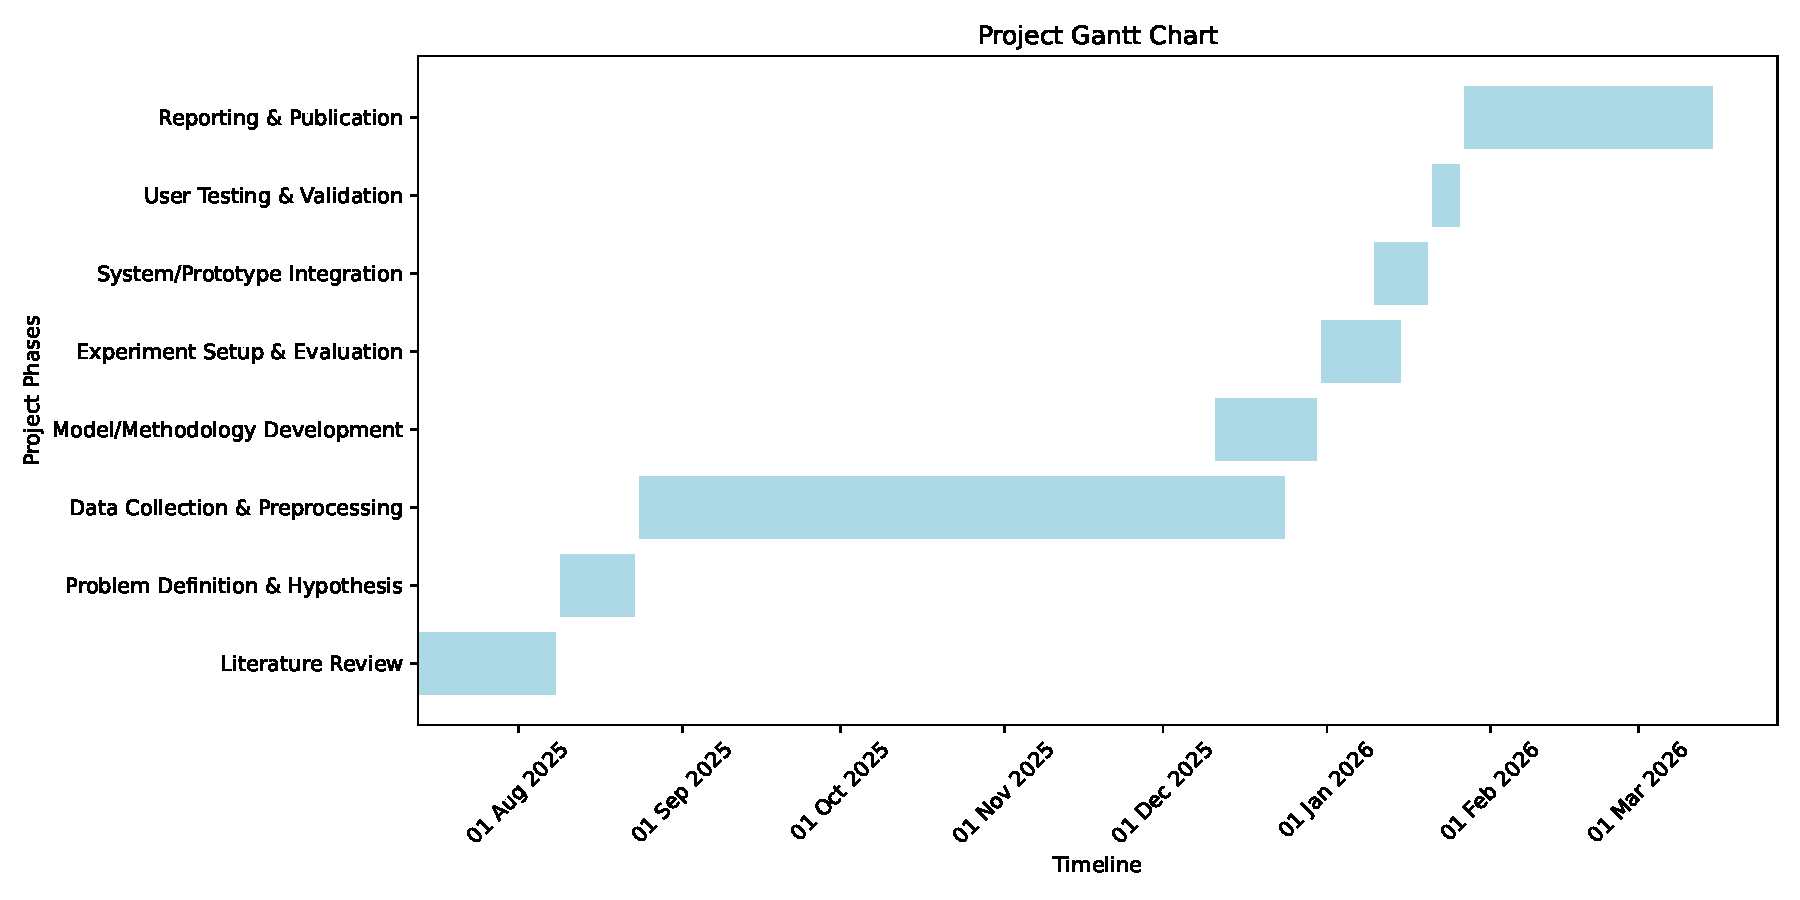
\includegraphics[width=\textwidth]{figures/gantt_chart_lightblue.pdf}
\caption{Gantt Chart of Project Timeline}
\label{fig:gantt-chart}
\end{figure}

\subsection{Financial Statement}

No specialized hardware was procured: all experiments ran on an existing CPU-only machine (Intel i3-6006U, no GPU) with commodity cameras, open-source software (Python, FFmpeg, YOLOv8n weights, Node.js, Next.js), and locally assembled datasets. The project therefore incurred no significant hardware or licensing cost.

\subsubsection{Budget Justification}

The zero-procurement budget is justified by the deployment scenario itself: the system is designed for low-cost, CPU-only operation, so developing and evaluating it on exactly such hardware strengthens rather than weakens the validity of the reported behaviour.


% Create Chapter 10: Ethical Consideration
\chapter{ETHICAL CONSIDERATION}
% Insert Ethical Consideration chapter content from external file
\section{Key Ethical Considerations}

\subsection{Informed Consent}

All thesis evaluation clips (\texttt{day\_person}, \texttt{day\_empty}, \texttt{night}, \texttt{motion\_only}, \texttt{crowd}) were recorded by the project team for the stated research purpose. Public datasets (CDnet-2014, UCF-Crime) were used under their released research terms. No covert recording of unaware subjects was conducted for this thesis.

\subsection{Data Security}

Event frames and manifests are stored locally with SHA-256 integrity chains (Chapter~6). The privacy-mode profile provides background blurring, face masking, and ethical frame-dropping (suppression of frames without ROI), reflecting the dual use of ROI machinery for privacy protection noted in prior work \cite{Ma2016Lossless}. Deployment handling of credentials, stream encryption, and access control is documented as operator responsibility and was not security-audited in this work.

\subsection{Fairness and Bias Mitigation}

The detector (YOLOv8n) and the heuristic risk weights were not tested for demographic or contextual bias, and no fairness claim is made. The risk score is a hand-tuned function of object counts, motion, time, and density; any deployment must assess disparate impact before operational use.

\subsection{Transparency}

All four evaluation phases record provenance (command, commit, hardware, configuration), report negative results (notably the Phase~4 matched-bitrate outcome and the withheld BD-rate), and demote superseded exploratory figures. No metric was selectively omitted to improve the narrative.

\subsection{Accountability}

The authors accept responsibility for the implemented system and for the accuracy of the evidence traceability claimed in this book. Every numerical result cites its evidence file; anything not traceable is labelled as not available in the current evidence.

\section{Demonstration of Ethical Awareness}

Surveillance technology concentrates power over observed subjects. This project treats that asymmetry as a design constraint: privacy modes, local processing at the edge, and tamper-evident (rather than tamper-proof-claiming) integrity reflect an attempt to build oversight into the pipeline, consistent with chain-of-evidence thinking \cite{Kanwal2020Chain}.

\section{Commitment to Responsible Research Practices}

No result was fabricated, exaggerated, or silently assumed. Where evidence was insufficient---generalization of calibration, legal admissibility of manifests, server performance---the thesis states the boundary explicitly and proposes the future work that could lift it (Chapter~14).


% Create Chapter 11: SYSTEM PERFORMANCE, SUSTAINABILITY AND SOCIETAL IMPACT
\chapter{SYSTEM PERFORMANCE, SUSTAINABILITY AND SOCIETAL IMPACT}
\section{Societal, Health, Safety, Legal and Cultural Aspects}

\subsection{Impact on Society}

Content-adaptive CCTV can lower the cost of public safety infrastructure and improve the usability of retained footage by protecting task-relevant regions \cite{Xiao2017Sensitive,Shao2018Smart}. Conversely, the same machinery could intensify pervasive monitoring if deployed without governance. This thesis takes no position on deployment policy beyond noting that efficiency gains do not by themselves justify expanded surveillance.

\subsection{Health and Safety Implications}

No physical intervention, human trial, or safety-critical control loop is involved. The system is a passive monitoring and compression pipeline; operator fatigue effects of adaptive quality (e.g.\ background degradation during review) were not studied and are noted as future human-factors work.

\subsection{Legal Considerations}

The forensic chain demonstrates exact-byte tamper evidence only. It does not establish legal admissibility, evidentiary sufficiency, certification, or standards compliance, and must not be represented as such to any court or authority. Chain-of-custody validity in the legal sense requires procedural controls far beyond file hashing \cite{Kanwal2020Chain}.

\subsection{Cultural Sensitivity}

Camera placement, retention, and privacy-mode configuration must respect local norms and regulations. The privacy profile (blur, masking, ethical dropping) exists to support such adaptation but does not guarantee cultural appropriateness in any specific deployment.

\section{System Performance, Sustainability and Societal Impact}

\subsection{Model Performance Evaluation}

\begin{table}[H]
\centering
\label{tab:performance_metrics}
\begin{tabular}{|l|c|l|}
\hline
\textbf{Metric} & \textbf{Value} & \textbf{Interpretation} \\
\hline
Phase~2 full descriptive AUC & 0.9962 & In-sample separability only, not generalization \\
Phase~2 full descriptive F1 & 0.919 & Apparent (all positives from one video) \\
Phase~3 localization recall / precision & 1.0 / 1.0 & 5/5 direct tampers; exact-byte scope \\
Phase~4 matched ROI-PSNR (proposed) & $\approx$ 31.5 dB & Below uniform $\approx$ 34.7 dB: negative result \\
Phase~4 BD-rate & Withheld & Preconditions not met; not reported \\
Detector consistency (Phase~4) & 1.0 & Internal consistency, not accuracy \\
\hline
\end{tabular}
\caption{Summary of measured performance (all values traceable to Chapters~4 and 7 evidence)}
\end{table}

\subsection{Sustainability}

CPU-only operation, open-source tooling, and reduced bitrate operation all favour lower energy and hardware cost relative to GPU-dependent learned codecs \cite{Wu2024ROIDVC,Zhao2025ASVC}. No energy measurement is claimed: power figures would require RAPL/instrumented metering that was not performed, and wall-clock runtime ($\approx$ 3.5 hours for Phase~4) is reported as runtime, not as energy or FPS.

\subsection{Broader Societal Impact (Positive and Negative)}

Positive: a reproducible, low-cost prototype with honest evaluation that other student and practitioner teams can build on. Negative: any compression system that degrades background regions risks discarding exculpatory or contextual detail; ROI-based evidence handling must therefore be paired with retention policies and the integrity mechanisms of Chapter~6, whose limits are stated plainly.


% Create Chapter 12: SOCIETAL, HEALTH, SAFETY, LEGAL AND CULTURAL ASPECTS
\chapter{SOCIETAL, HEALTH, SAFETY, LEGAL AND CULTURAL ASPECTS}
% Insert SOCIETAL, HEALTH, SAFETY, LEGAL AND CULTURAL ASPECTS chapter content from external file
\input{"chapters/chapter12_societal_health_safety_legal and_cultural_aspects"}

% Create Chapter 13: LIFELONG LEARNING AND SELF-DEVELOPMENT
\chapter{LIFELONG LEARNING AND SELF-DEVELOPMENT}
% Insert LIFELONG LEARNING AND SELF-DEVELOPMENT chapter content from external file
\section{Skills Developed}

This project required the integration of computer vision (YOLOv8n detection, ROI geometry, temporal persistence), video coding (FFmpeg, HEVC, GOP/bitrate control, PSNR/SSIM/VMAF metrology), full-stack development (Python edge services, Node.js/Express servers, Next.js dashboards), experimental methodology (frozen protocols, provenance recording, group-aware splitting, pre-registered forensic expectations, BD-rate withholding criteria), and academic writing under strict evidence discipline, including the reporting of negative results.

\section{Challenges Faced and Overcome}

The principal challenges were methodological rather than purely technical: concentrating all calibration positives in one video forced an honest degeneracy analysis instead of a headline metric; the foreground/background split's collapse on moving-camera content forced a negative-result narrative instead of a success story; and insufficient rate--distortion overlap forced BD-rate to be withheld rather than resurrected from older logs. Each was resolved by weakening the claim to match the evidence, which is the central professional lesson of the work.

\section{Applications of Learning}

The evidence-discipline practices adopted here---provenance files, evidence matrices, claim audits, number-consistency checks, and explicit NOT AVAILABLE markings---transfer directly to any future engineering or research role in which measurements inform decisions.

\section{Future Goals}

The authors intend to carry forward the combination of deployable building and honest evaluation: extending the ROI construction (e.g.\ motion-compensated backgrounds, learned priors \cite{Zhao2025ASVC}), validating on broader scene sets, and pursuing the calibration and forensic extensions listed in Chapter~14.


% Create Final Chapter: Conclusion
\chapter{CONCLUSION}
% Insert Conclusion chapter content from external file
\section{Conclusion}

This thesis designed, implemented, and evaluated an adaptive CCTV compression system using dynamic ROI control. RQ1 is answered affirmatively as a construction result: a deployable YOLOv8n/FFmpeg edge-cloud prototype with heuristic risk scoring (NORMAL/ALERT/CRITICAL), Lagrangian-inspired ROI allocation, 15-second pre-event and 10-second post-event buffering with SHA-256 hash-chained manifests, and a Next.js monitoring dashboard was built and documented with all evaluated parameters. RQ2 is answered descriptively: the risk score tracks detected-object/ROI importance across CDnet-2014 and UCF-Crime probes (e.g.\ highway risk $\approx$ 0.563, pedestrians $\approx$ 0.492, night $\approx$ 0.024; Normal\_050 $\approx$ 0.994 versus Fighting002 $\approx$ 0.068), while group-aware calibration over 64 labelled seconds shows in-sample separability (descriptive AUC $\approx$ 0.9962, F1 $\approx$ 0.919) without established generalization. RQ3 is answered negatively: under the locked same-codec protocol, the current ROI construction did not outperform uniform encoding at matched bitrate (proposed ROI-PSNR $\approx$ 31.5 dB versus uniform $\approx$ 34.7 dB at $\approx$ 710--840 kbps), with BD-rate withheld. RQ4 is answered positively within scope: the event buffer demonstrated exact-byte tamper-evident integrity behaviour (5/5 direct tampers detected, zero clean-case false alarms) without any legal-admissibility claim. The overall contribution is therefore a deployable YOLOv8n/FFmpeg edge-cloud CCTV prototype with heuristic risk scoring, Lagrangian-inspired ROI allocation, and tamper-evident event buffering, evaluated through public-dataset probing, group-aware calibration analysis, controlled forensic tests, and a locked same-codec baseline comparison---with the current ROI construction's limitation stated as plainly as its capabilities.

\section{Limitations}

The work is limited by: a small calibration set with positives from a single video; single-class LOVO folds and one degenerate fold; hour-fixing in Phase~1; a single primary motion clip in Phase~4; a limited tamper-operation set with exact-byte scope and no legal validation; CPU-only execution with no energy or FPS claims; no independent detector ground truth in Phase~4 (consistency, not accuracy); withheld BD-rate; the dropped-hysteresis deviation of Phase~4 from the live system; and no systematic server/dashboard performance evaluation. Superseded exploratory figures (e.g.\ -87.95\%/-83.15\% BD-rate, 20.4 FPS, 217 kbps, 0.913 SSIM, greater than 95\% recall as a headline) are demoted and not claimed.

\section{Future Work}

Future work should: (i) redesign the ROI construction for moving-camera content (motion-compensated or learned backgrounds \cite{Zhao2025ASVC,Wu2024ROIDVC}, adaptive dilation, per-region QP optimization against ROI-weighted distortion); (ii) extend evaluation to more scenes, codecs (including AV1/VP9 paths already in the harness), and longer sequences with overlapping rate--distortion coverage sufficient for valid BD-rate computation; (iii) collect multi-video calibration labels so that generalization---not just apparent fit---can be tested under LOVO; (iv) broaden forensic testing (more tamper types, robustness-oriented integrity such as perceptual hashing) while preserving the exact-byte baseline; (v) re-examine the risk/anomaly relationship with frame-level anomaly annotations rather than clip labels, informed by the anomaly literature \cite{Duong2023Survey,ACMTaxonomy2024,Baradaran2021Anomaly}; and (vi) evaluate server/dashboard performance and energy consumption with instrumented metering. Each direction builds directly on the prototype and protocols documented in this book.


% ===============================
% REFERENCES
% ===============================
% Start the reference section on a new page
\clearpage

% Include all bibliography entries even if they are not cited in the document
\nocite{*}
% Add the reference section manually to the Table of Contents
\addcontentsline{toc}{chapter}{REFERENCE}
% Rename the bibliography heading from the default name to "REFERENCE"
\renewcommand{\bibname}{REFERENCE}
% Use IEEE citation and bibliography formatting style
\bibliographystyle{IEEEtran}
% Load bibliography entries from the references.bib file
\bibliography{references}
% ===============================
% APPENDIX
% ===============================
% Switch the document to appendix mode
% Chapter numbering changes from numbers (1, 2, 3...) to letters (A, B, C...)
\appendix
% Insert Appendix A content from the external file
\chapter{APPENDIX A: SUPPLEMENTARY EVIDENCE}

\section{Parameter Reference}

All evaluated parameters are listed in Table~\ref{tab:params} (Chapter~6). Deployment presets are listed in Table~\ref{tab:profiles} (Chapter~5). The full risk-score definition is Equation~\ref{eq:risk} (Chapter~4).

\section{Evidence Matrix (Claim $\rightarrow$ Experiment $\rightarrow$ Evidence File)}

\begin{longtable}{@{}lll@{}}
\textbf{Claim / result} & \textbf{Experiment} & \textbf{Evidence file} \\
Phase~1 CDnet risks/agreement & Phase~1 & phase1\_public/cdnet\_scene\_results.csv \\
Phase~1 UCF risks/rates & Phase~1 & phase1\_public/ucf\_video\_results.csv \\
514 inferences, 0 skipped/failed & Phase~1 & phase1\_public/provenance.json \\
LOVO folds, coefficients & Phase~2 & phase2\_calibration/calibration\_results.json \\
AUC 0.9962, F1 0.919 (descriptive) & Phase~2 & phase2\_calibration/calibration\_metrics.csv \\
ROC/PR and reliability plots & Phase~2 & roc\_pr\_full\_apparent.png, reliability\_full.png \\
Forensic cases and localization & Phase~3 & phase3\_forensics/cases.csv, localization.csv \\
Phase~4 RD points (all methods) & Phase~4 & phase4\_sota/roi\_metrics.csv, runs.csv \\
Matched-bitrate table & Phase~4 & phase4\_sota/matched\_bitrate.csv \\
BD-rate withheld & Phase~4 & phase4\_sota/bd\_diagnostics.json \\
Fairness lock and runtime 9764\,s & Phase~4 & phase4\_sota/provenance.json \\
RD curves & Phase~4 & rd\_psnr.png, rd\_roi.png, rd\_bg.png \\
\end{longtable}

\section{Reference--Citation Matrix (Reference $\rightarrow$ Section $\rightarrow$ Claim Supported)}

All 45 references are cited in Chapter~2 (Sections 2.1--2.8) by theme: standards and early surveillance compression (Section~2.2); classical/heuristic ROI (2.3); object-aware and foreground/background methods (2.4); edge-cloud analytics (2.5); recognition-aware and adaptive allocation including VCM (2.6); learned and recent adaptive coding (2.7); forensic chain of evidence (2.8); anomaly detection context (2.9). Method chapters cite the directly supporting works (ROI practice in Chapters~4--6; forensic framing in Chapters~6 and 10; literature comparison figures in Chapter~7; future-work directions in Chapters~13--14). No reference is cited for a result it did not report; literature figures (e.g.\ -32\%, -50.4\%, -49.75\%, 25.0--76.9\%, -74.63\%) are attributed strictly as author-reported results on their own protocols.

\section{Visual Insertion Checklist}

\begin{longtable}{@{}llll@{}}
\textbf{No.} & \textbf{Title} & \textbf{Location} & \textbf{Status / action} \\
Fig.~4.1 & Conceptual pipeline (TikZ) & Ch.~4 & Inserted (TikZ source) \\
Fig.~5.1 (placeholder) & Deployment architecture & Ch.~5 & NEW FIGURE REQUIRED \\
Fig.~5.2 & Risk-state machine (TikZ) & Ch.~5 & Inserted (TikZ source) \\
Fig.~6.1 (placeholder) & YOLO/ROI overlay example & Ch.~6 & NEW FIGURE REQUIRED \\
Fig.~7.1 & Phase~2 ROC/PR & Ch.~7 & Inserted (phase2\_roc\_pr.png) \\
Fig.~7.2 & Phase~2 reliability & Ch.~7 & Inserted (phase2\_reliability.png) \\
Fig.~7.3 & Hash-chain diagram (TikZ) & Ch.~7 & Inserted (TikZ source) \\
Fig.~7.4 (placeholder) & Tampering example frame & Ch.~7 & AVAILABLE --- NEEDS FORMATTING \\
Fig.~7.5 & Phase~4 RD global & Ch.~7 & Inserted (phase4\_rd\_psnr.png) \\
Fig.~7.6 & Phase~4 RD ROI & Ch.~7 & Inserted (phase4\_rd\_roi.png) \\
Fig.~7.7 & Phase~4 RD background & Ch.~7 & Inserted (phase4\_rd\_bg.png) \\
Fig.~8.1--8.2 (placeholder) & Dashboard screenshots & Ch.~8 & NEW SCREENSHOT REQUIRED \\
Fig.~9.1 & Gantt chart & Ch.~9 & Inserted (existing PDF) \\
Tabs.~4.1--7.6, 11.1 & All result tables & inline & Inserted with evidence values \\
\end{longtable}

\section{Claim Audit (Residual Items Requiring Manual Verification)}

\begin{itemize}
\item Student names, IDs, supervisor, examiners, and degree statements on the title/declaration/approval pages must be verified against departmental records.
\item Dashboard screenshots (Figures~8.1--8.2), the deployment architecture diagram (Figure~5.1), the ROI overlay example (Figure~6.1), and the tamper-example export (Figure~7.4) must be created or captured before final printing.
\item The Gantt chart file (\texttt{figures/gantt\_chart\_lightblue.pdf}) is inherited from the template and must be replaced with the actual project timeline if the department requires it.
\item Bibliographic details of the 45 references (supplied DOI/URL strings) should be spot-checked against publisher records before submission.
\item No numerical claim remains unverified beyond these presentation items: every in-text number traces to the evidence matrix above.
\end{itemize}


\end{document}